\documentclass[conference]{IEEEtran}
\IEEEoverridecommandlockouts
% The preceding line is only needed to identify funding in the first footnote. If that is unneeded, please comment it out.
\usepackage{cite}
\usepackage{amsmath,amssymb,amsfonts}
\usepackage{algorithmic}
\usepackage{graphicx}
\usepackage{textcomp}
\usepackage{xcolor}
\usepackage[utf8]{inputenc}
\usepackage[vietnamese]{babel}
\usepackage{amsmath}
\usepackage{float} 
\usepackage{booktabs}
\usepackage{multirow}
\usepackage[table]{xcolor}
\usepackage{tabularx} % For adjusting table width
\usepackage{longtable} % For tables that span multiple pages
\usepackage{adjustbox}
\usepackage{changepage}
\usepackage{xcolor}
\usepackage{booktabs}
\usepackage{array}
\usepackage{makecell}
\usepackage{titlesec}
% Đặt margin top và bottom
\titlespacing{\section}{0pt}{5pt}{2pt}
\titlespacing{\subsection}{0pt}{2pt}{2pt}
\setlength{\abovedisplayskip}{10pt}
\setlength{\belowdisplayskip}{10pt}
\setlength{\abovedisplayshortskip}{5pt}
\setlength{\belowdisplayshortskip}{0pt}


\def\BibTeX{{\rm B\kern-.05em{\sc i\kern-.025em b}\kern-.08em
    T\kern-.1667em\lower.7ex\hbox{E}\kern-.125emX}}
\begin{document}

\title{Dự đoán giá của ba loại nhiên liệu ở Hoa Kì sử dụng các kĩ thuật phân tích chuỗi thời gian\\
}

\author{\IEEEauthorblockN{1\textsuperscript{st} Lê Thị Thanh Hằng}
\IEEEauthorblockA{\textit{Trường đại học Công nghệ thông tin
 } \\
\textit{IS403.021}\\
21520222@gm.uit.edu.vn}
\and
\IEEEauthorblockN{2\textsuperscript{nd} Ngô Tất Tố}
\IEEEauthorblockA{\textit{Trường đại học Công nghệ thông tin} \\
\textit{IS403.021}\\
21520484@gm.uit.edu.vn}
\and
\IEEEauthorblockN{3\textsuperscript{rd} Nguyễn Nhật Phương Huy}
\IEEEauthorblockA{\textit{Trường đại học Công nghệ thông tin} \\
\textit{IS403.021}\\
21522156@gm.uit.edu.vn}
\and
\hspace{2.5cm}
\IEEEauthorblockN{4\textsuperscript{th} Lê Xuân Thạch}
\IEEEauthorblockA{\hspace{2.5cm}\textit{Trường đại học Công nghệ thông tin} \\
\hspace{2.5cm}\textit{IS403.021}\\
\hspace{2.5cm}21521421@gm.uit.edu.vn}
\and
\IEEEauthorblockN{5\textsuperscript{th} Hô Quang Đỉnh}
\IEEEauthorblockA{\textit{Trường đại học Công nghệ thông tin} \\
\textit{IS403.021}\\
21520190@gm.uit.edu.vn}
}

\maketitle

\begin{abstract}
Nghiên cứu này đi sâu vào việc dự đoán giá của Heating Oil, Crude Oil WTI, Gasoline RBOB bằng cách sử dụng một loạt các thuật toán máy học và học sâu đa dạng. Chúng tôi sử dụng các mô hình Hồi quy tuyến tính, AIRMA, RNN, GRU, LSTM, FFT, DLM, FCN để đo độ chính xác và đáng tin cậy của các dự báo được tạo ra bởi mỗi thuật toán.
\end{abstract}

\begin{IEEEkeywords}
Time series analysis, Energy market investment, Forecasting gasoline and oil prices, machine learning, deep learning, LR, ARIMA, RNN, GRU, LSTM, FFT, DLM, FCN.\end{IEEEkeywords}

\section{Giới Thiệu}
Báo cáo này tập trung vào việc dự đoán giá cả trên thị trường dầu khí, tập trung vào ba loại dầu khí lớn: Heating Oil, Crude Oil WTI và Gasoline RBOB. Sử dụng các phương pháp phân tích chuỗi thời gian tiên tiến trên dữ liệu lịch sử, nghiên cứu nhằm mục đích phát hiện các mẫu và xu hướng giúp hiểu rõ hơn về biến động giá trong tương lai.

Mục đích của nghiên cứu này là hỗ trợ các nhà đầu tư, nhà phân tích tài chính và những người làm chính sách trong việc đưa ra quyết định thông minh về quản lý rủi ro, chiến lược đầu tư và kế hoạch tài chính.

Trong quá trình nghiên cứu, chúng tôi áp dụng một loạt các mô hình phân tích và dự đoán gồm Hồi quy Tuyến tính, ARIMA, RNN, GRU, LSTM, FFT, DLM, FCN và addRNN. Mỗi mô hình đều mang lại những ưu điểm riêng, giúp phân tích chi tiết các động lực phức tạp ảnh hưởng đến biến động giá cả của các loại dầu khí này.


\section{Các nghiên cứu liên quan}
Trong lĩnh vực dự đoán giá cổ phiếu , nhiều nghiên cứu quan trọng đã được tiến hành với các mô hình học máy. Dự đoán giá cổ phiếu trong tương lai là một nhiệm vụ khó khăn do sự ngẫu nhiên cao trong biến động giá. Nghiên cứu của C. C. Emioma1 và S. O. Edeki1 nhằm sử dụng một thuật toán học máy để ước tính giá đóng cửa của cổ phiếu từ một tập dữ liệu, nhằm tăng độ chính xác trong việc dự đoán giá cổ phiếu. Mô hình này được dự định sử dụng như một hướng dẫn giao dịch trong ngày. Thuật toán được sử dụng là mô hình hồi quy tuyến tính theo phương pháp bình phương nhỏ nhất. Nó sử dụng biến phụ thuộc là giá đóng cửa của cổ phiếu và biến độc lập là ngày mà mỗi giá cổ phiếu được ghi nhận. \cite{b1}. 
Cũng trong lĩnh vực dự đoán giá cổ phiếu, Chris Kuo/Dr. Dataman đã sử đụng cả ba mô hình RNN/LSTM/GRU áp dụng ARIMA để dự đoán được giá cổ phiếu \cite{b2}. Và với mô hình khác như Random Forest trong nghiên cứu của các trang blog \cite{b3}.\\
Ta thấy được thị trường tài chính có vai trò quan trọng trong sự phát triển của xã hội hiện đại. Họ cho phép triển khai các nguồn lực kinh tế. Những thay đổi về giá cổ phiếu phản ánh những thay đổi trên thị trường. Trong nghiên cứu tập trung vào việc dự đoán giá cổ phiếu bằng mô hình học sâu Jialin Liu, Fei Chao, Yu-Chen Lin và Chih-Min Lin đã sử dụng các mô hình học sâu FCN -LSTM để dự đoán giá cổ phiếu \cite{b4}.
Và trong báo cáo khác của Hassan Ismail Fawaz, Germain Forestier, Jonathan Weber, Lhassane Idoumghar, Pierre-Alain Muller về việc sử dụng học sâu để dự đoán cho chuỗi thời gian \cite{b5}.\\
Một số nghiên cứu sử dụng các mô hình trong vòng bốn mươi năm qua, sự phát triển của các mô hình Độ dẻo Tinh thể (Crystal Plasticity - CP) và các thuật toán của chúng (CP-FEM) đã chuyển hóa kiến thức về cơ học vật lý ở mức hệ thống trượt thành các mô hình cấu tạo cho các vật liệu đơn và đa tinh thể. Các nghiên cứu gần đây đã tập trung vào việc tăng hiệu suất tính toán của CP-FEM thông qua thuật toán Biến đổi Fourier Nhanh (FFT) và sử dụng mạng nơ-ron hồi quy (RNN) để mô phỏng phản ứng ứng suất-biến dạng của vật liệu. Các mô hình này giúp tăng tốc độ tính toán đáng kể mà vẫn duy trì độ chính xác của các mô phỏng tiêu chuẩn \cite{b6}.\\
Trong nghiên cứu khác dự đoán chính xác thời gian di chuyển là một tính năng quan trọng để hỗ trợ Hệ thống Giao thông Thông minh (ITS). Tuy nhiên, tính phi tuyến của của Semin Kwak và Nikolas Geroliminisnày \cite{b7} đề xuất sử dụng mô hình tuyến tính động (DLM) để xấp xỉ các trạng thái giao thông phi tuyến. Khác với mô hình hồi quy tuyến tính tĩnh, DLM giả định rằng các tham số của nó thay đổi theo thời gian. 
\section{Bộ dữ liệu}
\subsection{Nguồn dữ liệu}
- Bộ dữ liệu này bao gồm giá bán trong ngày của 3 loại nhiên liệu phổ biến: Heating Oil,Crude Oil WTI, Gasoline RBOB tại Hoa Kỳ từ 1/1/2019 đến 27/3/2024. Dữ liệu được thu thập từ trang web investing.com, một nguồn tin cậy và uy tín trong lĩnh vực tài chính. Bảng I mô tả các cột có trong bộ dữ liệu.

- Mô tả các thành phần của tập dữ liệu:
\begin{table}[h!]
    \centering
        \caption{Bảng mô tả thành phần của tập dữ liệu}
    \renewcommand\arraystretch{1.5} % Điều chỉnh chiều dọc của bảng
    \begin{adjustbox}{max width=\linewidth}
    \begin{tabular}{|>{\centering}m{2.5cm}|m{7cm}|}
        \hline
        \textbf{Tên Cột} & \textbf{Ý Nghĩa} \\
        \hline
        Date  & Ngày dữ liệu được ghi nhận \\
        \hline
        Price  & Giá cuối cùng của ngày giao dịch đó \\
        \hline
        Open  & Giá đầu tiên được giao dịch trong ngày đó \\
        \hline
        High  & Giá cao nhất được giao dịch trong ngày \\
        \hline
        Low  & Giá thấp nhất được giao dịch trong ngày \\
        \hline
        Vol (volume)  & Tổng số lượng nhiên liệu được giao dịch trong ngày \\
        \hline
        Change \%  & Phần trăm thay đổi giữa giá cuối cùng của ngày dữ liệu ghi nhận so với ngày trước đó \\
        \hline
    \end{tabular}
    \end{adjustbox}
    \label{tab:data_description}
\end{table}
\subsection{Thống kê mô tả}
\begin{table}[H]
  \centering
  \caption{Heating Oi, Crude Oil WTI, Gasoline RBOB’s Descriptive Statistics}
\begin{tabular}{|>{}c|c|c|c|}
    \hline
      & HT Oil& WTI& RBOB\\ \hline
     Count & 1320
& 1322
& 1550
\\ \hline
     Mean & 2.351011
& 68.126384
& 1.946561
\\ \hline
     Std & 0.846315
& 20.452117
& 0.590874
\\ \hline
     Min & 0.6104
& -37.63
& 0.543
\\ \hline
     25\% & 1.8314
& 55.705
& 1.411925
\\ \hline
     50\% & 2.15365
& 70.015
& 1.9412
\\ \hline
     75\% & 2.891425
& 80.5
& 2.44925
\\ \hline
     Max & 5.1354
& 123.7
& 4.3144
\\ \hline
 Mode& 3.3622
& 47.62
&2.581
\\\hline
 Median& 2.15365
& 70.015
&1.9412
\\\hline
 Var& 0.716249
& 418.289074
&0.349132
\\\hline
 Kurtosis& -0.39922
& 0.452915
&-0.377936
\\\hline
 Skewness& 0.389108
& -0.09777
&0.261192
\\\hline
 CV& 0.359979
& 0.300208
&0.303548
\\\hline
\end{tabular}
\end{table}

\begin{figure}[H]
    \centering
    \begin{minipage}{0.23\textwidth}
    \centering
    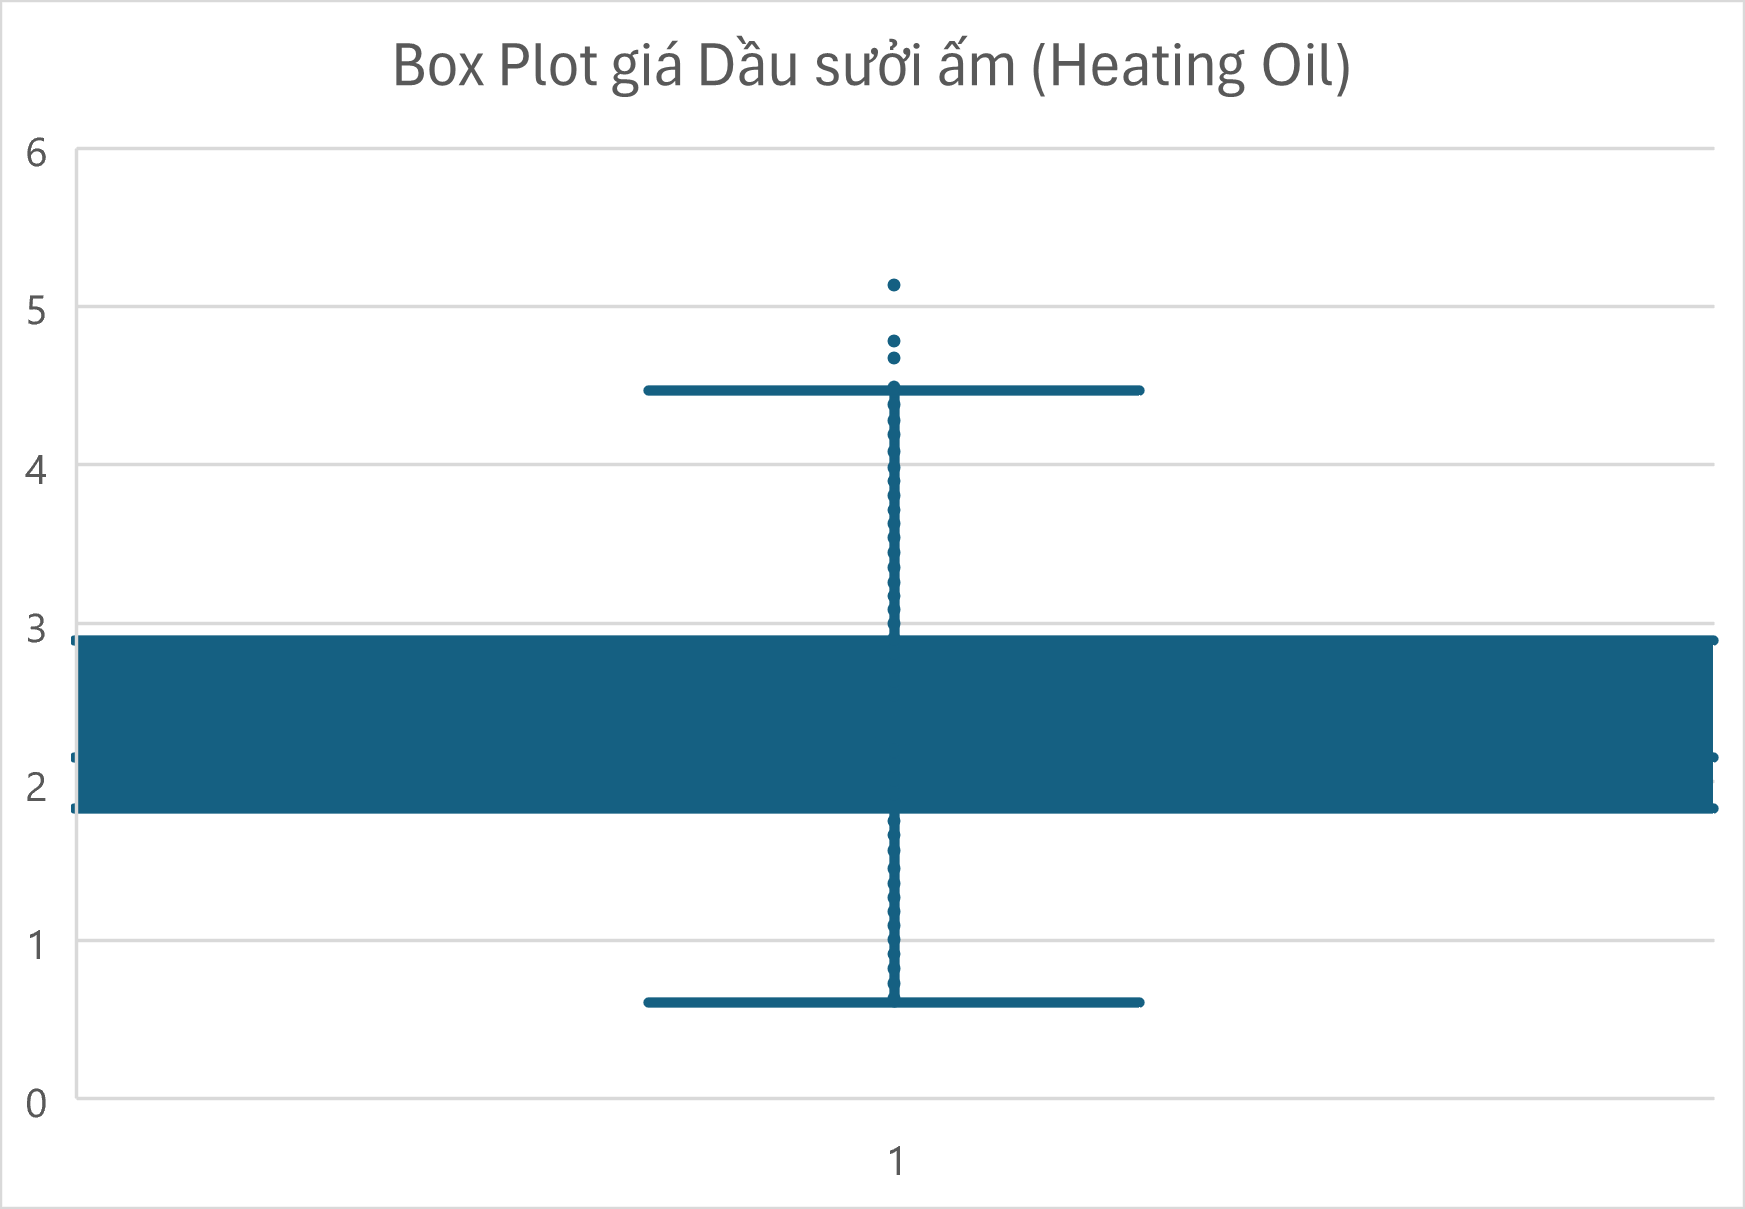
\includegraphics[width=1\textwidth]{Picture/BoxPlot cho phần III/Team9_Box_HeatingOil.png}
    \caption{Box Plot giá Dầu sưởi ấm (Heating Oil)}
    \label{fig:1}
    \end{minipage}
    \hfill
    \begin{minipage}{0.23\textwidth}
    \centering
    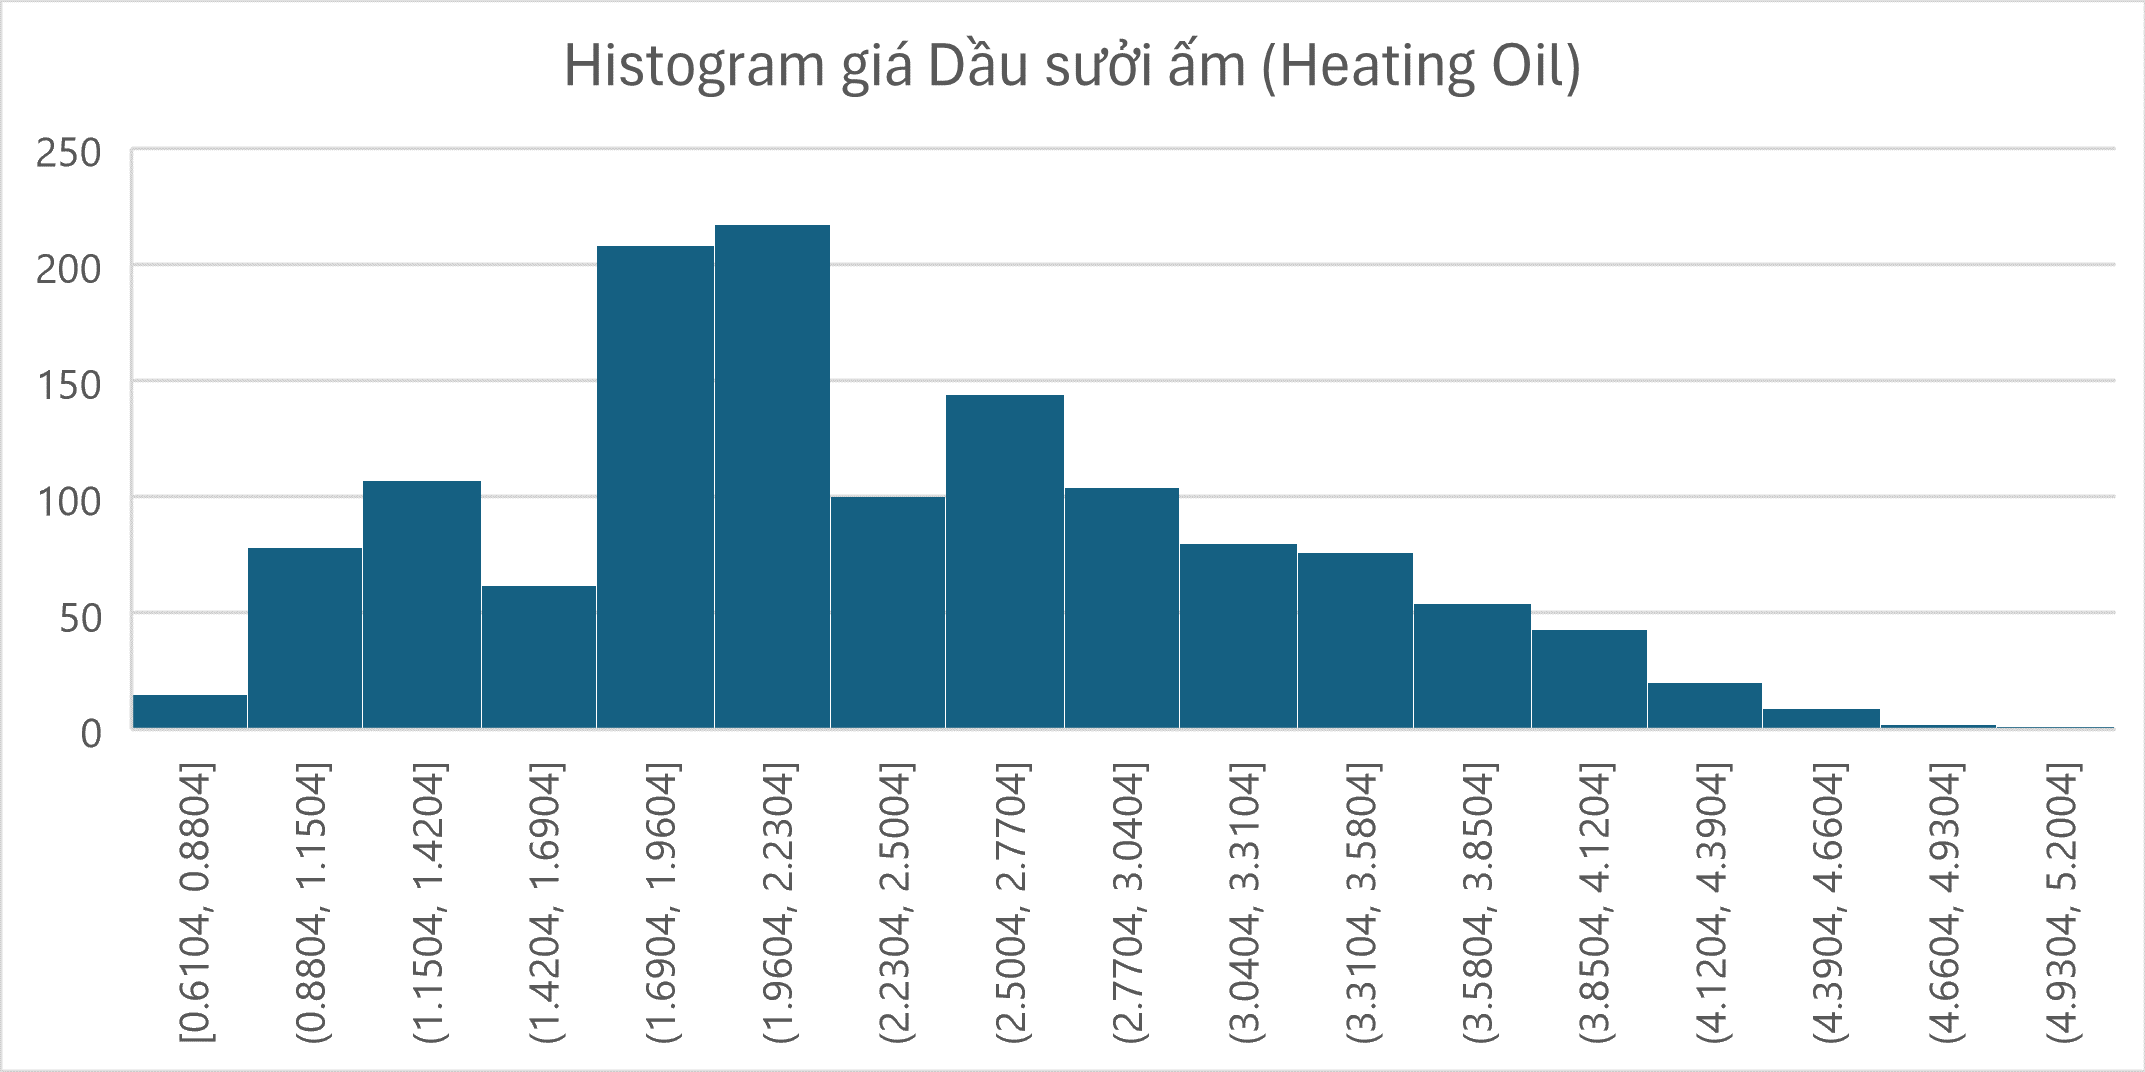
\includegraphics[width=1\textwidth]{Picture/Histogram cho ở phần III/Team9_His_HeatingOil.png}
    \caption{Histogram giá Dầu sưởi ấm (Heating Oil)}
    \label{fig:2}
    \end{minipage}
\end{figure}

\begin{figure}[H]
    \centering
    \begin{minipage}{0.23\textwidth}
    \centering
    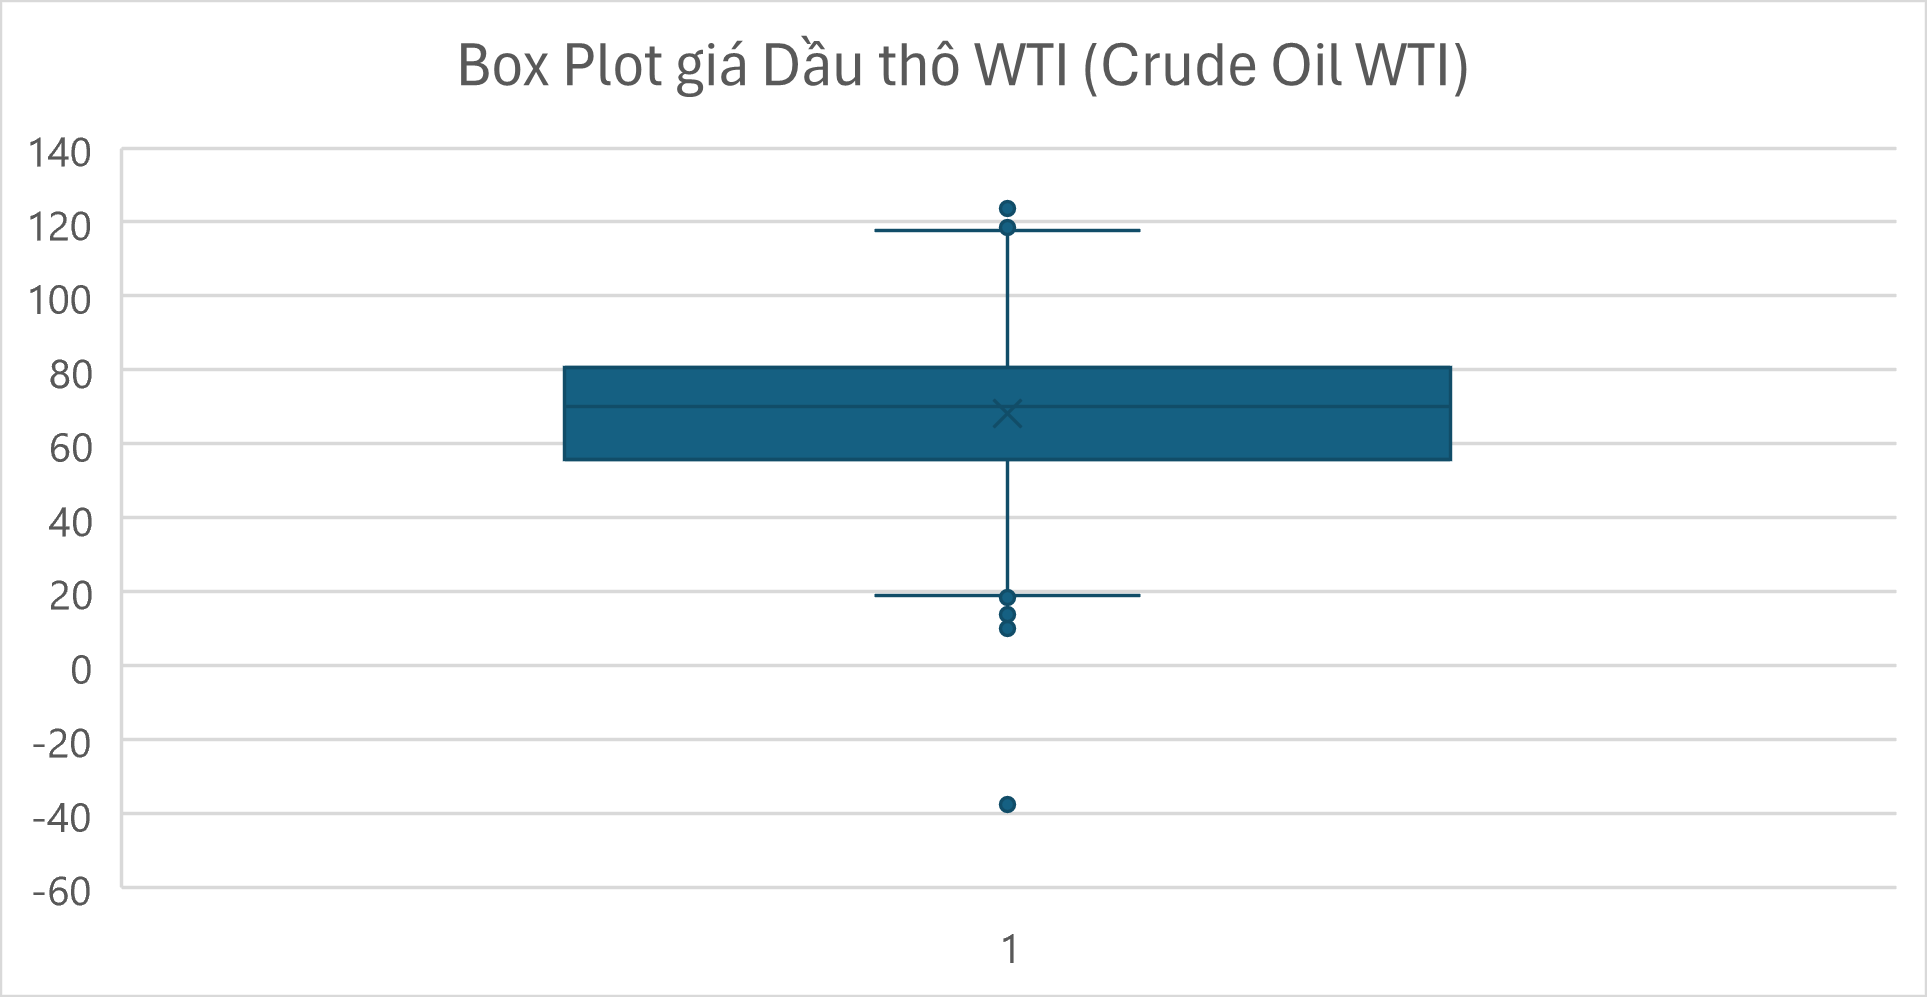
\includegraphics[width=1\textwidth]{Picture/BoxPlot cho phần III/Team9_Box_WTI.png}
    \caption{Boxplot giá Dầu thô WTI (Crude Oil WTI}
    \label{fig:1}
    \end{minipage}
    \hfill
    \begin{minipage}{0.23\textwidth}
    \centering
    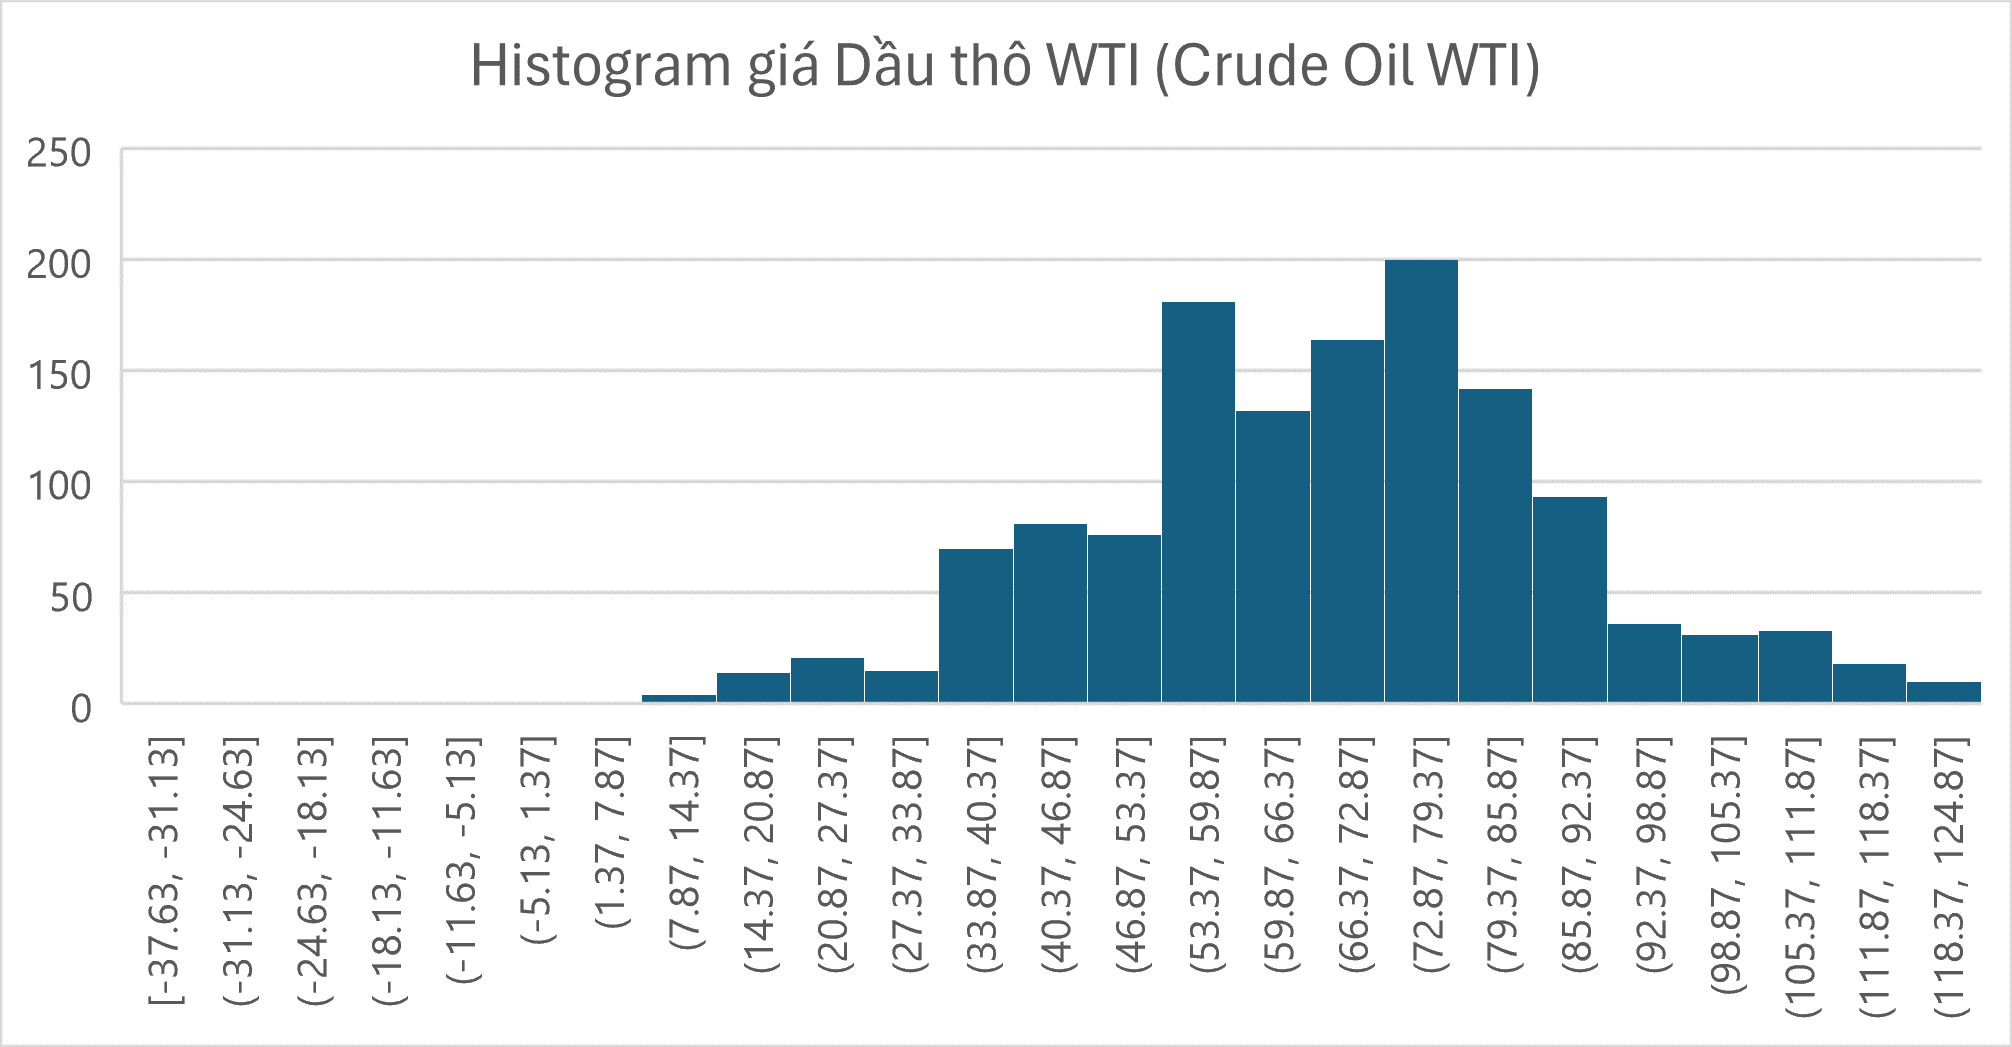
\includegraphics[width=1\textwidth]{Picture/Histogram cho ở phần III/Team9_His_WTI.png}
    \caption{Histogram giá Dầu thô WTI (Crude Oil WTI)}
    \label{fig:2}
    \end{minipage}
\end{figure}

\begin{figure}[H]
    \centering
    \begin{minipage}{0.23\textwidth}
    \centering
    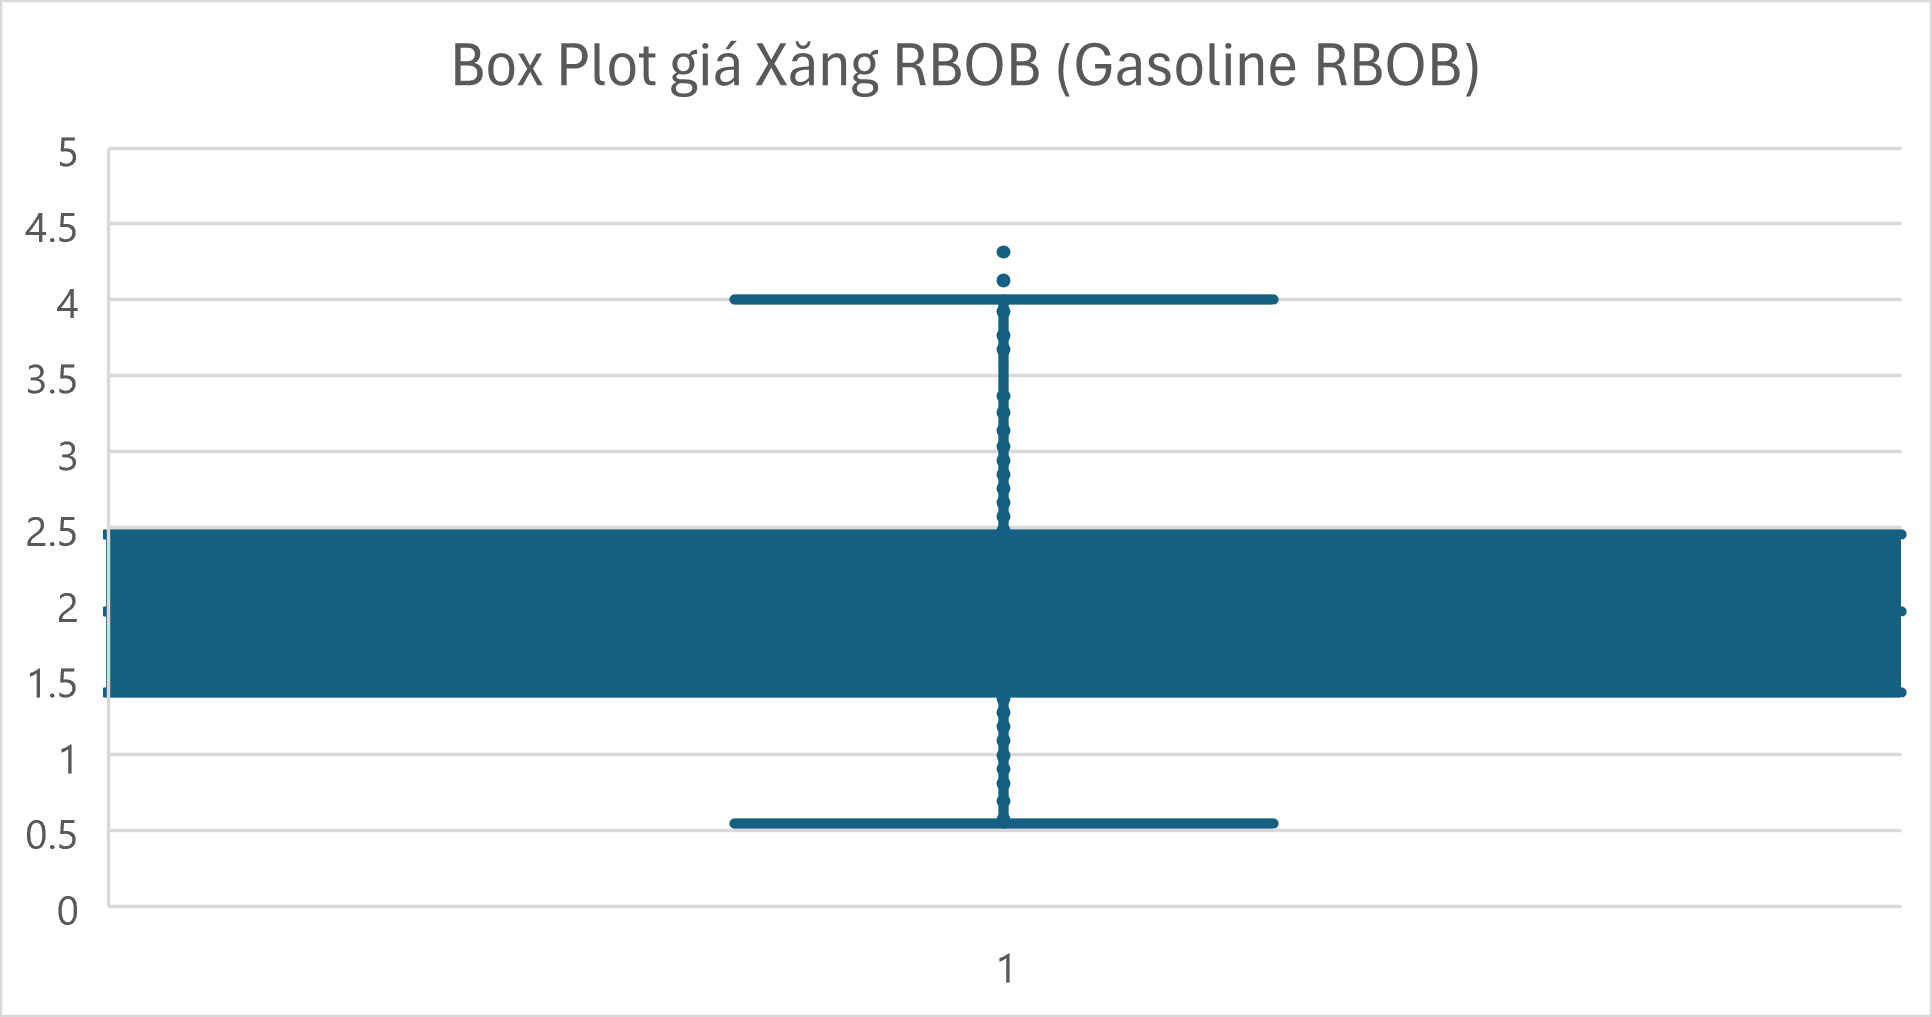
\includegraphics[width=1\textwidth]{Picture/BoxPlot cho phần III/Team9_Box_RBOB.png}
    \caption{Boxplot giá Xăng RBOB (Gasoline RBOB)}
    \label{fig:1}
    \end{minipage}
    \hfill
    \begin{minipage}{0.23\textwidth}
    \centering
    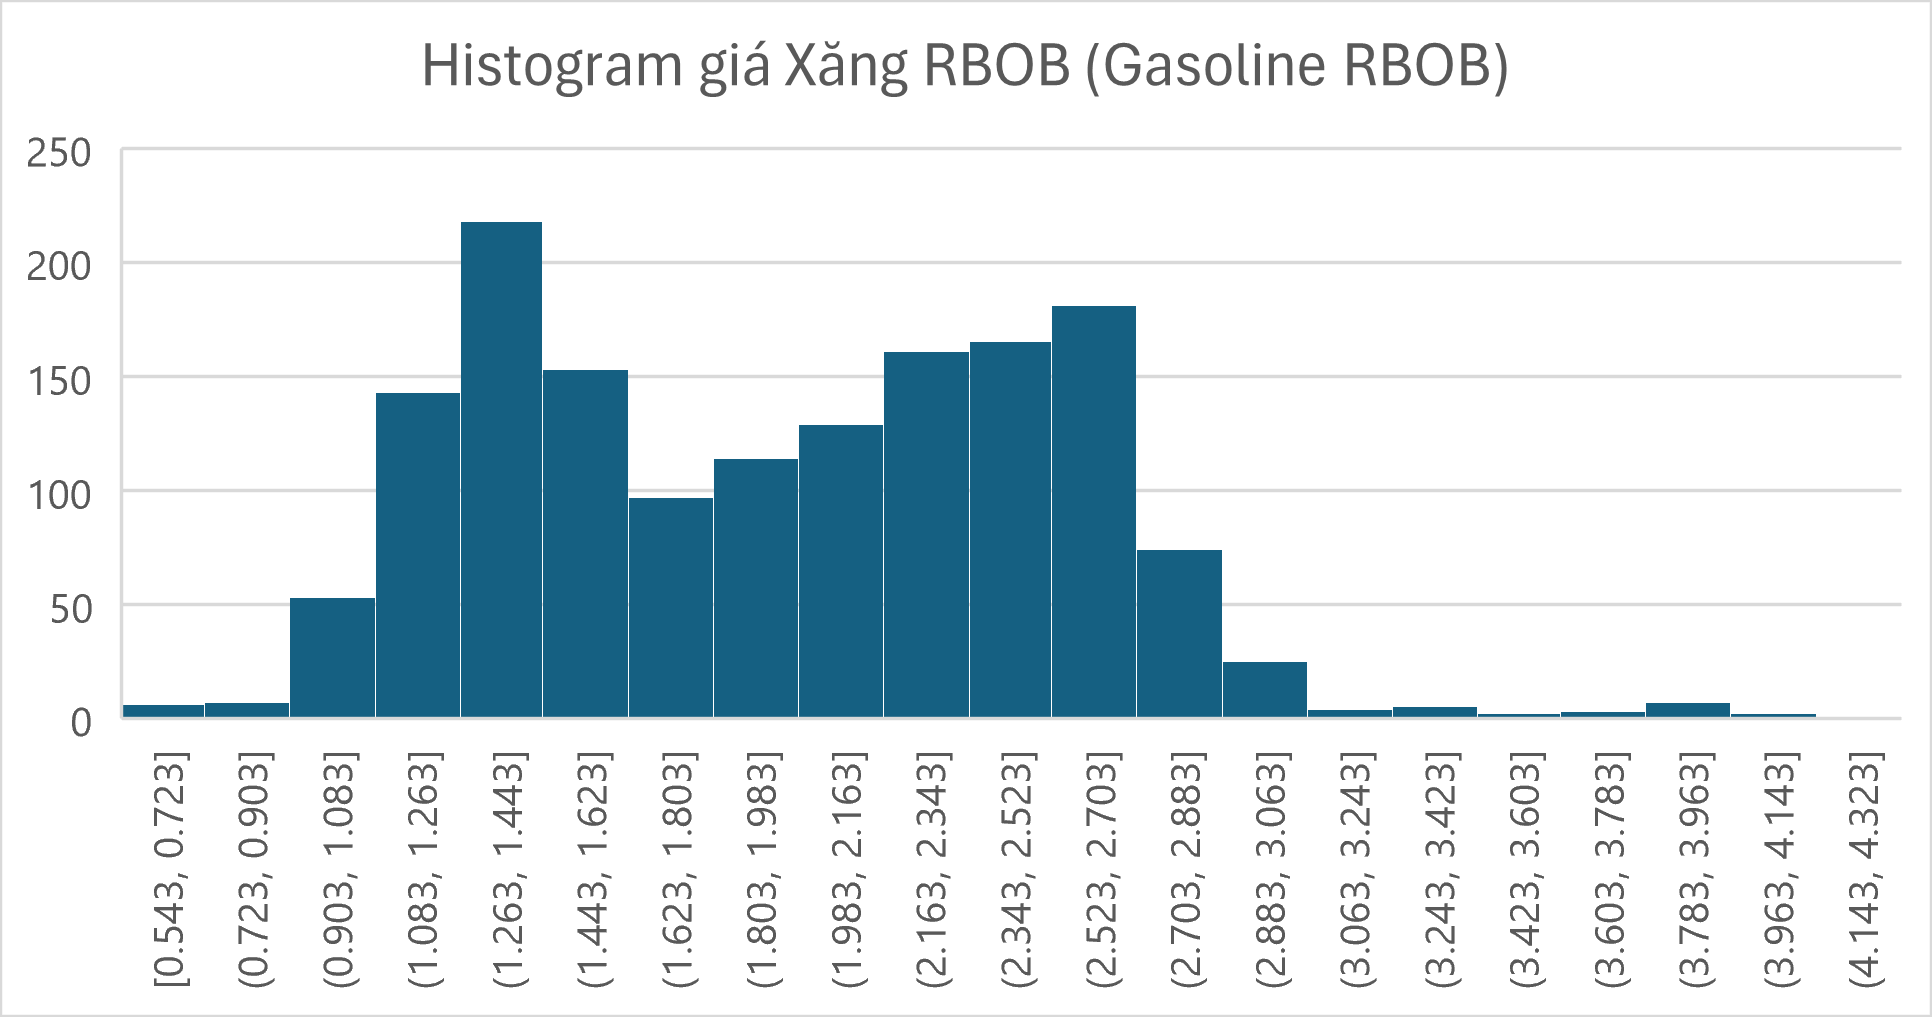
\includegraphics[width=1\textwidth]{Picture/Histogram cho ở phần III/Team9_His_RBOB.png}
    \caption{Histogram giá Xăng RBOB (Gasoline RBOB)}
    \label{fig:2}
    \end{minipage}
\end{figure}
\subsection{Công cụ}
Trong quá trình nghiên cứu và phân tích dữ liệu, nhóm đã sử dụng một bộ công cụ phân tích thống kê bằng Python để hiểu sâu hơn về các mẫu dữ liệu và rút ra ý nghĩa, kết luận. Các công cụ chính bao gồm: numpy, pandas, sklearn, matplotlib.pyplot,...


\subsection{Tỉ lệ phân chia dữ liệu}
    Trong việc phân tích dữ liệu chuỗi thời gian, nhóm đã chia tập dữ liệu thành các tập huấn luyện và kiểm tra bằng các tỷ lệ khác nhau: 70\% cho huấn luyện và 30\% cho kiểm tra, 80\% cho huấn luyện và 20\% cho kiểm tra, 90\% cho huấn luyện và 10\% cho kiểm tra. 

Những tỷ lệ này cho phép đánh giá tác động của các chỉ số liên quan đến hiệu suất của mô hình bằng cách xem xét phân phối dữ liệu trong mỗi tập. Tỷ lệ phổ biến 7:3 phân bổ 70\% cho huấn luyện và 30\% cho kiểm tra, tạo ra một sự cân bằng giữa cung cấp đủ dữ liệu huấn luyện, đồng thời đảm bảo sự khác nhau giữa các tập cho việc điều chỉnh và đánh giá. Một lựa chọn khác là tỷ lệ 8:2, ưu tiên tập huấn luyện 80\%, có lợi cho các mô hình phức tạp yêu cầu một tập dữ liệu huấn luyện lớn hơn. Hoặc một cách phân tích thận trọng dùng tỷ lệ 9:1 có thể được ưa chuộng, khi xử lý một tập dữ liệu lớn và một mô hình đơn giản. Tỷ lệ này đảm bảo dữ liệu huấn luyện và vẫn đủ dữ liệu một tập kiểm tra để đánh giá hiệu suất.

\subsection{Đánh giá mô hình}
RMSE được tính bằng cách lấy căn bậc hai của trung bình cộng bình phương của các sai số (khác biệt giữa giá trị dự đoán và giá trị thực tế) giữa một loạt các điểm dữ liệu. RMSE càng nhỏ thì mô hình dự đoán càng chính xác [8].

MAPE được tính bằng cách lấy trung bình cộng của tỷ lệ tuyệt đối giữa sai số tuyệt đối và giá trị thực tế cho mỗi điểm dữ liệu, sau đó nhân 100 để biểu diễn dưới dạng phần trăm [9].

MAE được tính bằng cách lấy trung bình cộng của các giá trị tuyệt đối của sai số giữa giá trị dự đoán và giá trị thực tế [10].

\[RMSE=\sqrt{\sum_{i=1}^{n} \frac{(\hat{y_i}-y_i )^2}{n} }\]\\

\[MAPE = \frac{1}{n} \sum_{i=1}^{n} \left| \frac{y_i - \hat{y_i}}{y_i} \right| \times 100\]\\

\[MAE = \frac{1}{n} \sum_{i=1}^{n} \left| y_i - \hat{y_i} \right|]\\

Trong đó \(n\) là số lượng các điểm dữ liệu, \(y_i\) là các giá trị thực tế của điểm dữ liệu thứ i, và \(\hat{y_i}\) là các giá trị dự đoán tương ứng.
\section{Phương pháp thống kê}
\subsection{Linear Regression}
Phân tích hồi quy là một phân tích thống kê để xác định xem quan hệ các biến độc lập quy định các biến phụ thuộc như thế nào.\\
Hồi quy tuyến tính là một công cụ dùng để xây dựng các mô hình toán học và thống kê, mô tả mối quan hệ giữa biến phụ thuộc và một hoặc nhiều biến độc lập (hoặc biến giải thích), tất cả đều là các biến số.Mô hình hồi quy tuyến tính này được sử dụng để tìm phương trình dự đoán tốt nhất cho biến y dưới dạng một hàm tuyến tính của các biến x\\

Mô hình hồi quy tuyến tính bội có dạng: 
\[
Y=\beta_0+\beta_1X_1+\beta_2X_2+\cdots+\beta_kX_k+\varepsilon
\]
Định nghĩa: Y là biến phụ thuộc (biến mục tiêu), \(X_1, X_2, \ldots, X_k\) là các biến độc lập (biến giải thích), \(\beta_0\) là giá trị trung bình của biến phụ thuộc khi \(X = 0\), và \(\beta_1, \ldots, \beta_k\) là các hệ số cho các biến độc lập, với \(\varepsilon\) là sai số của mô hình.

\begin{figure}[H]
    \centering
    \begin{minipage}{0.3\textwidth}
    \centering
    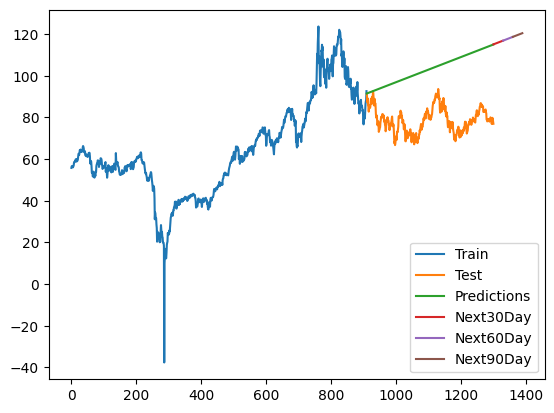
\includegraphics[width=0.8\textwidth]{Picture/LinearRegression/LN_Cruide_7_3.png} 
    \caption{Crude Oil WTI 7:3}
    \label{fig:1}
    \end{minipage}
    \hfill
    \\
    \begin{minipage}{0.3\textwidth} 
    \centering
    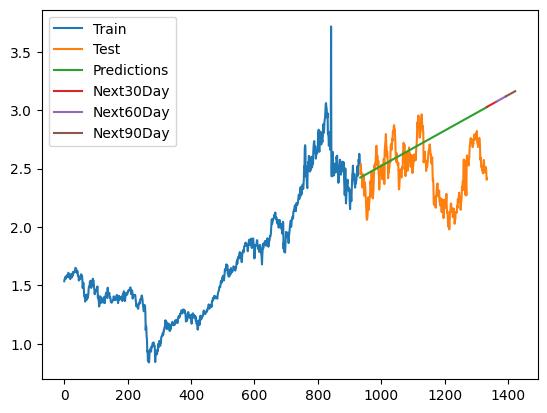
\includegraphics[width=0.8\textwidth]{Picture/LinearRegression/LN_Gao_7_3.png} 
    \caption{Gasoline RBOB 7:3}
    \label{fig:2}
    \end{minipage}
    \hfill
    \\
    \begin{minipage}{0.3\textwidth}
    \centering
    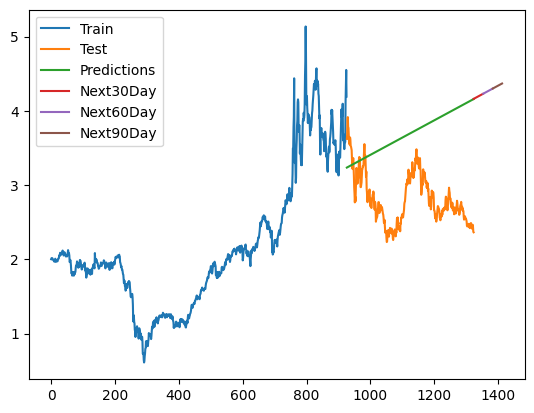
\includegraphics[width=0.8\textwidth]{Picture/LinearRegression/LN_Heating_7_3.png}
    \caption{Heating Oil 7:3}
    \label{fig:3}
    \end{minipage}
\end{figure}

\subsection{ARIMA}
 ARIMA (Auto-Regressive Integrated Moving-Average) là mô hình phân tích thống kê sử dụng dữ liệu chuỗi thời gian để hiểu rõ hơn về tập dữ liệu hoặc để dự đoán xu hướng trong tương lai. Trong phần này sẽ đề cập về ARIMA không có tính mùa vụ (Non-seasonal).
 Mô hình ARIMA không có tính mùa vụ (Non-seasonal) được kí hiệu là ARIMA(p,d,q) với p, d, q là các số không âm. Trong đó, ARIMA bao gồm 3 phần:
 \textbf{AR(p)} - \textit{Auto-Regression}: là quá trình tìm mối quan hệ giữa dữ liệu hiện tại và \textbf{\textit{p}} dữ liệu trước đó (hay còn gọi là lag). 
 Mô hình AR(p) có dạng:
 \[y_t = \alpha_0 + \alpha_1 y_{t-1} + \alpha_2 y_{t-2} + \cdots + \alpha_p y_{t-p} + \varepsilon_t\]
Trong đó, điều kiện dừng của việc chọn \textbf{\textit{p}} là: $\sum_{i=0}^{p} \alpha_i < 1$ \\
\textbf{MA(q)} - \textit{Moving-Average}: là quá trình tìm mối quan hệ giữa dữ liệu hiện tại và \textbf{\textit{q}} phần lỗi trước đó. Mô hình MA(q) có dạng: 
\[y_t = \beta_0 + \beta_1 \varepsilon_{t-1} + \beta_2 \varepsilon_{t-2} + \cdots + \beta_q \varepsilon_{t-q} + \mu_t\]
 Trong đó, điều kiện dừng của việc chọn 
 \textbf{\textit{q}} là: $\sum_{i=0}^{q} \beta_i < 1$ \\
 \textbf{I(d)} - \textit{Integrated}: là quá trình đồng tích hợp hoặc lấy sai phân. Để tạo thành chuỗi dừng cho mô hình ARMA, một cách đơn giản nhất là lấy sai phân (I - Integrated) để tạo thành mô hình ARIMA. 
 Với \textbf{\textit{d}} là số chênh lệch cần thiết cho tính dừng (hiệu giữa giá trị hiện tại và \textbf{\textit{d}} giá trị trước đó).
 Quá trình sai phân bậc \textbf{\textit{d}} (hoặc \textbf{\textit{d}} lần lấy sai phân) của chuỗi được thực hiện như sau:\\
 Sai phân bậc 1 - I(1): $\Delta y_t = y_t - y_{t-1}$  \\
 Sai phân bậc 2 - I(2): $\Delta(\Delta y_t) = (y_t - y_{t-1}) - (y_{t-1} - y_{t-2}) $ \\
 Sai phân bậc \textbf{\textit{d}} - I(d): $\Delta^d (x_t)$
\begin{figure}[H]
    \centering
    \begin{minipage}{0.3\textwidth}
    \centering
    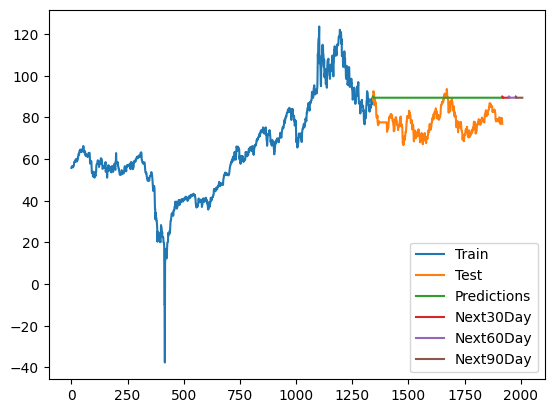
\includegraphics[width=0.8\textwidth]{Picture/ARIMA/Crude Oil WTI 7_3.png} 
    \caption{Crude Oil WTI 7:3}
    \label{fig:1}
    \end{minipage}
    \hfill
    \\
    \begin{minipage}{0.3\textwidth} 
    \centering
    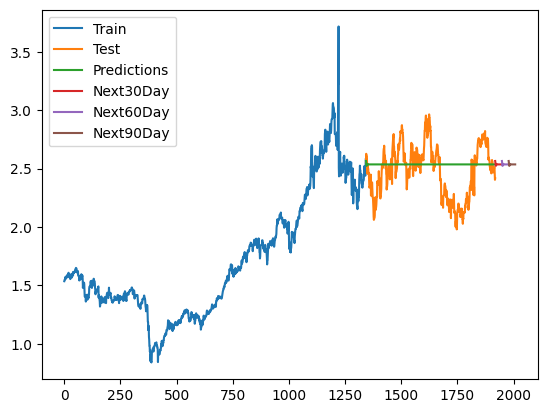
\includegraphics[width=0.8\textwidth]{Picture/ARIMA/Gasoline RBOB 7_3.png} 
    \caption{Gasoline RBOB 7:3}
    \label{fig:2}
    \end{minipage}
    \hfill
    \\
    \begin{minipage}{0.3\textwidth}
    \centering
    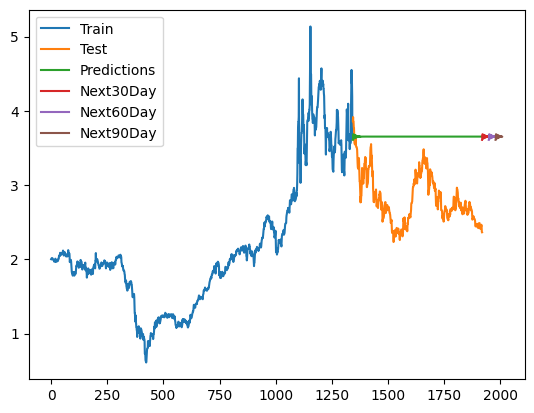
\includegraphics[width=0.8\textwidth]{Picture/ARIMA/Heating Oil 7_3.png}
    \caption{Heating Oil 7:3}
    \label{fig:3}
    \end{minipage}
\end{figure}

\subsection{Fast Fourier Transform Forecasting Model (FFT)}

Fast Fourier Transform - FFT là một thuật toán được sử dụng để dự đoán các giá trị dữ liệu trong tương lai. Thuật toán này biến đổi Fourier rời rạc của một dãy hoặc nghịch đảo của nó, thường thì cả hai đều được thực hiện. Phân tích Fourier biến đổi tín hiệu từ miền của dữ liệu đã cho, thường là thời gian hoặc không gian, và biến đổi nó thành biểu diễn tần số.
Công thức của thuật toán FFT:
\[
X_k = \sum_{m=0}^{N/2-1} x_{2m}e^{-\frac{2\pi i}{N}mk} + \sum_{m=0}^{N/2-1} x_{2m+1}e^{-\frac{2\pi i}{N}(m+N/2)k}
\]
Trong đó, \( X_k \) là giá trị của Fourier tại vị trí \( k \), \( x_m \) là giá trị của điểm dữ liệu trong dữ liệu đầu vào tại vị trí \( m \), \( N \) là kích thước của dữ liệu đầu vào, \( e \) là số Euler, một hằng số toán học (\( e \approx 2.71828 \)), và \( i \) là đơn vị ảo trong toán học.
\begin{figure}[H]
    \centering
    \begin{minipage}{0.3\textwidth}
    \centering
    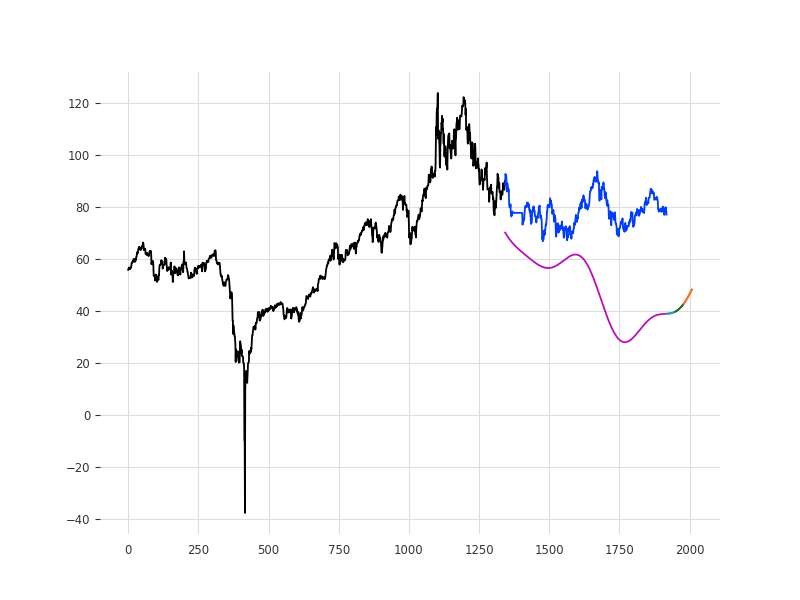
\includegraphics[width=0.8\textwidth]{Picture/FFT/FFT_Crude_73.png} 
    \caption{Crude Oil WTI 7:3}
    \label{fig:1}
    \end{minipage}
    \hfill
    \\
    \begin{minipage}{0.3\textwidth} 
    \centering
    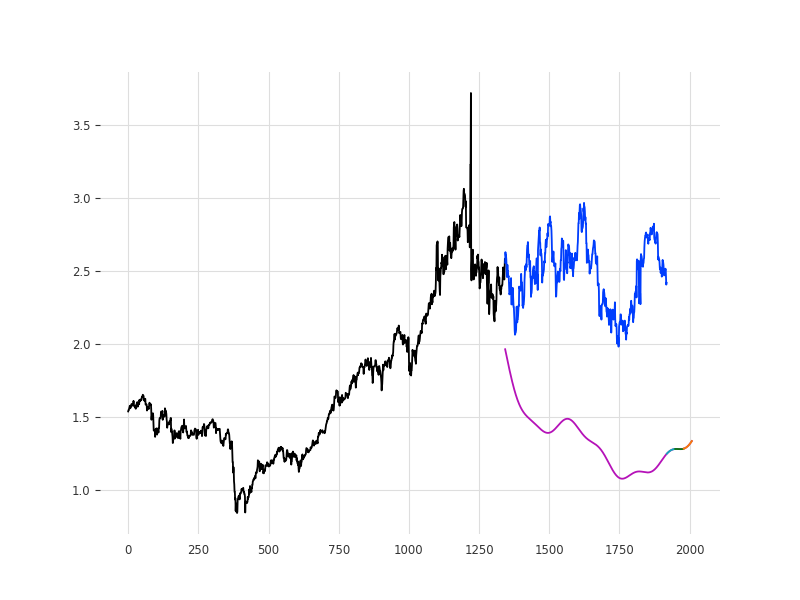
\includegraphics[width=0.8\textwidth]{Picture/FFT/FFT_Gasoline_73.png}
    \caption{Gasoline RBOB 7:3}
    \label{fig:2}
    \end{minipage}
    \hfill
    \\
    \begin{minipage}{0.3\textwidth}
    \centering
    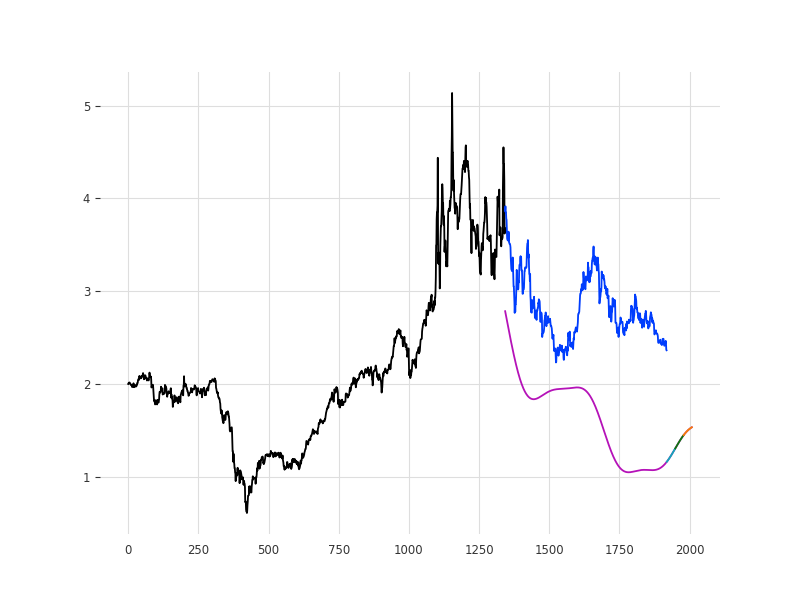
\includegraphics[width=0.8\textwidth]{Picture/FFT/FFT_Heating_73.png}
    \caption{Heating Oil 7:3}
    \label{fig:3}
    \end{minipage}
\end{figure}
\subsection{Recurrent Neural Network (RNN)}
Recurrent Neural Network (RNN) là một kiến trúc mạng nơ-ron nhân tạo trong Deep learning, được thiết kế để xử lý dữ liệu tuần tự hoặc chuỗi dữ liệu. RNN có khả năng lưu giữ trạng thái trước đó của một chuỗi đầu vào và sử dụng thông tin đó để tính toán đầu ra tiếp theo.
RNN có một số ưu điểm để dự đoán chuỗi thời gian (time-series). Chúng có thể xử lý dữ liệu theo chuỗi có độ dài khác nhau, nắm bắt hiệu quả các phụ thuộc lâu dài và mô hình thời gian. RNN dễ dàng thích ứng với các khoảng thời gian không đều nhau hay các tác vụ dự báo khác nhau với các chuỗi input và output có độ dài khác nhau.

Công thức mô hình trạng thái ẩn tại thời điểm \( t \):
\[ H_t = f(U \cdot X_t + W \cdot H_{t-1} + b) \]
Biết được trạng thái ẩn \( H_t \) của thời điểm hiện tại, công thức tính toán giá trị đầu ra dự đoán \( Y_t \) của RNN tại thời điểm hiện tại như sau: 
\[ Y_t = g(V \cdot H_t + c) \]
\\
Trong đó, \( X_t \) là đầu vào tại thời điểm \( t \), \( Y_t \) là đầu ra tại thời điểm \( t \), \( H_t \) là trạng thái ẩn tại thời điểm \( t \), \( U \) là ma trận trọng số liên kết giữa đầu vào và trạng thái ẩn, \( W \) là ma trận trọng số liên kết giữa trạng thái ẩn tại thời điểm trước đó và trạng thái ẩn tại thời điểm hiện tại, \( V \) là ma trận trọng số liên kết giữa trạng thái ẩn và đầu ra, \( b \) và \( c \) là vector độ lệch (bias), và \( f \) và \( g \) là hàm kích hoạt.

RNN sử dụng các thuật toán tối ưu hoá (Optimization algorithm) để tối thiểu hóa độ lỗi (loss) bằng cách cập nhật lại các tham số của mạng (bao gồm các ma trận trọng số và vector độ lệch) thông qua việc tính toán đạo hàm (Gradient) của hàm mất mát (Loss function) theo các tham số trên và di chuyển theo hướng ngược lại với gradient theo một tỷ lệ học (learning rate) xác định.
Quá trình này được lặp lại cho tất cả các chuỗi đầu vào trong quá trình huấn luyện mạng RNN.

\begin{figure}[H]
    \centering
    \begin{minipage}{0.3\textwidth}
    \centering    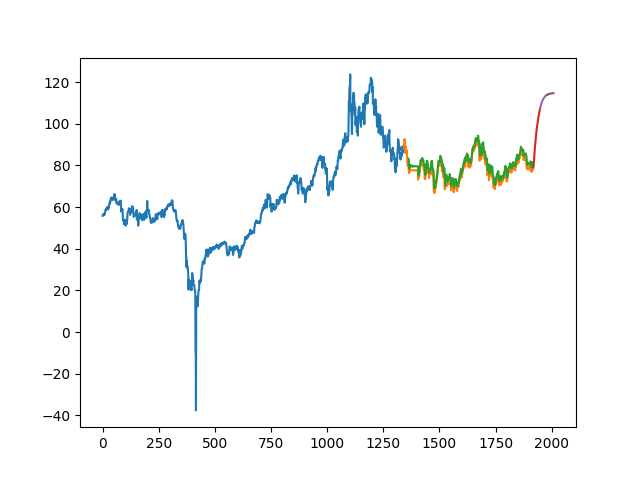
\includegraphics[width=0.8\textwidth]{Picture/RNN/RNN_Crude_73.png} 
    \caption{Crude Oil WTI 7:3}
    \label{fig:1}
    \end{minipage}
    \hfill
    \\
    \begin{minipage}{0.3\textwidth} 
    \centering
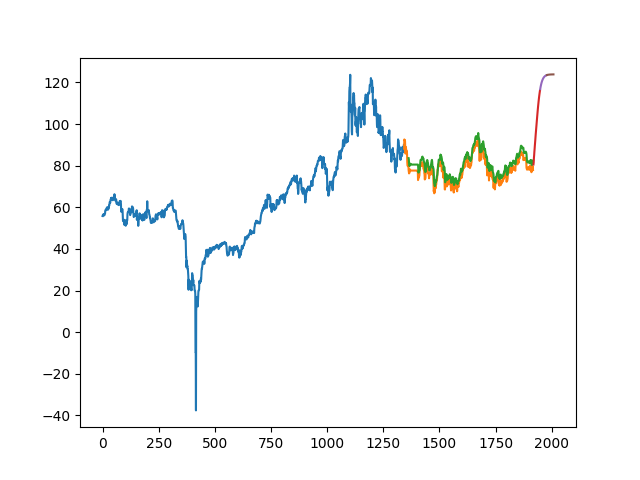
\includegraphics[width=0.8\textwidth]{Picture/RNN/RNN_Gasoline_73.png} 
    \caption{Gasoline RBOB 7:3}
    \label{fig:2}
    \end{minipage}
    \hfill
    \\
    \begin{minipage}{0.3\textwidth}
    \centering    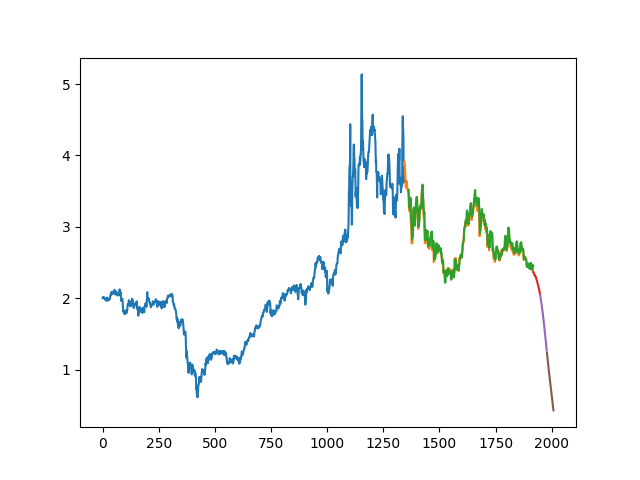
\includegraphics[width=0.8\textwidth]{Picture/RNN/RNN_Heating_73.png}
    \caption{Heating Oil 7:3}
    \label{fig:3}
    \end{minipage}
\end{figure}

\subsection{Random Forest (RF)}
Random Forest là một phương pháp học máy phổ biến, được sử dụng rộng rãi trong nhiều bài toán dự đoán. Về bản chất thì Random Forest là tập hợp của nhiều cây quyết định, thay vì phụ thuộc vào một cây, nó lấy kết quả từ mỗi cây và dựa trên đa số phiếu dự đoán, để đưa ra kết quả cuối cùng.

Dưới đây là sơ đồ minh họa cho mô hình Cây quyết định:

\begin{figure}[H]
    \centering
    \begin{minipage}{0.5\textwidth}
        \centering
        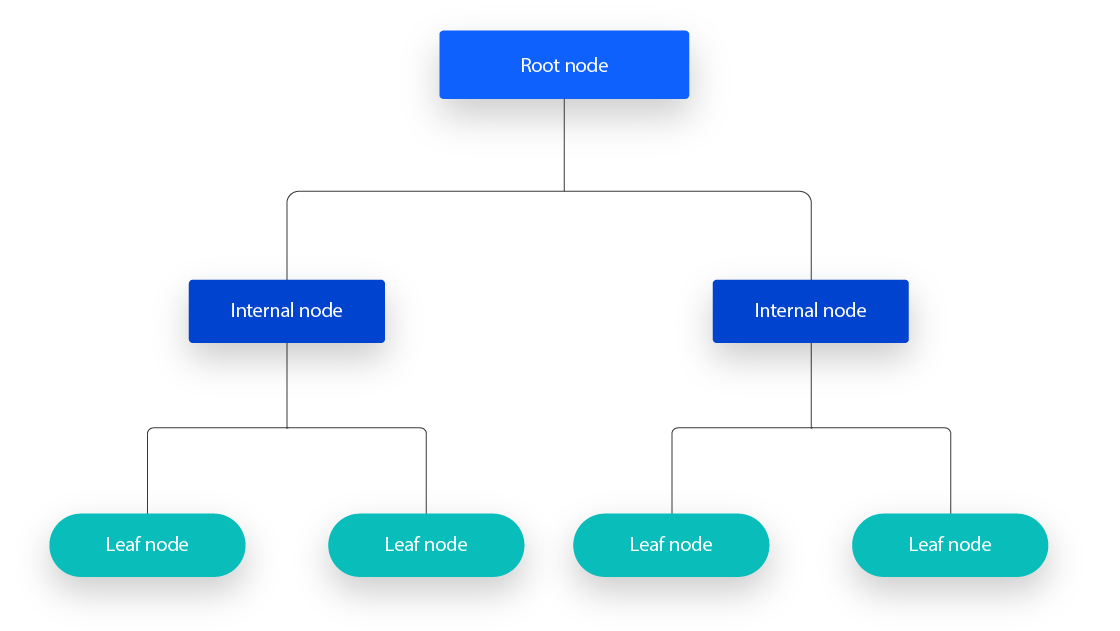
\includegraphics[width=\textwidth]{Picture/RF/Decision-Tree.png} 
        \caption{Mô hình cây quyết định (Decision Tree)}
        \label{fig:decision-tree}
    \end{minipage}
\end{figure}
Một cây quyết định bao gồm ba loại nút:
\begin{itemize}
    \item Nút quyết định: loại nút này có hai nhánh trở lên.
    \item Nút lá: các nút này đại diện cho các quyết định thấp nhất.
    \item Nút gốc: là nút quyết định ở mức cao nhất trong cây.
\end{itemize} 

Khi áp dụng mô hình Random Forest cho dữ liệu chuỗi thời gian, cần xem xét và xử lý đặc thù của loại dữ liệu này, chẳng hạn như tính phụ thuộc thời gian và cấu trúc tuần tự. Một phương pháp hiệu quả để xử lý vấn đề này là sử dụng biến thể của Random Forest với cơ chế "block bootstrap", giúp duy trì tính liên tục và mối quan hệ thời gian trong dữ liệu. khi sử dụng RandomForestRegressor trong Python với thư viện scikit-learn, tham số "bootstrap" mặc định là “True”.\\
Mô hình Random Forest kết hợp "block bootstrap" có dạng như sau:
\begin{figure}[H]
    \centering
    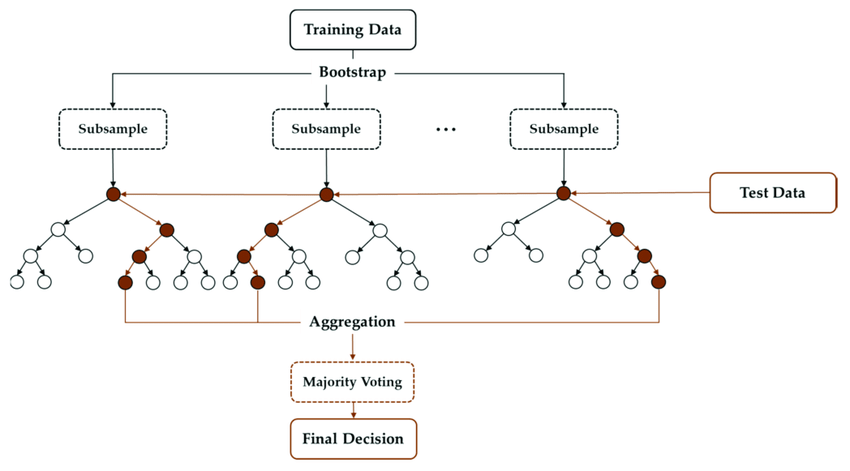
\includegraphics[width=0.5\textwidth]{Picture/RF/RF_BlockBootstrap.png} 
    \caption{Mô hình Random Forest với block bootstrap}
    \label{fig:rf-block-bootstrap}
\end{figure}
\begin{figure}[H]
    \centering
    \begin{minipage}{0.3\textwidth}
    \centering
    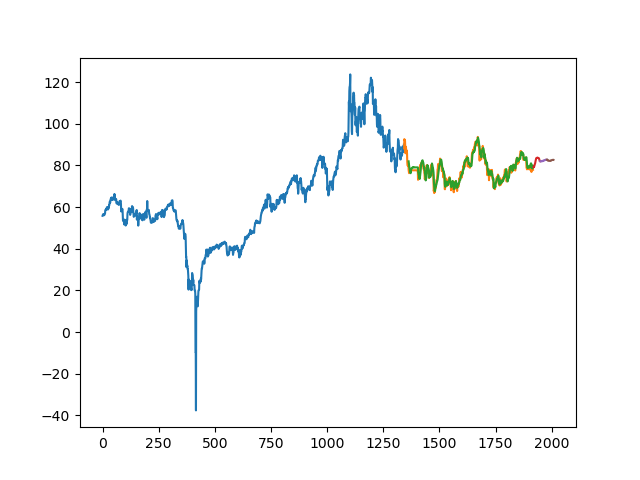
\includegraphics[width=0.8\textwidth]{Picture/RF/RF_Cruide_Oil_Week6.png} 
    \caption{RF Crude Oil WTI 7:3}
    \label{fig:1}
    \end{minipage}
    \hfill
    \\
    \begin{minipage}{0.3\textwidth} 
    \centering
    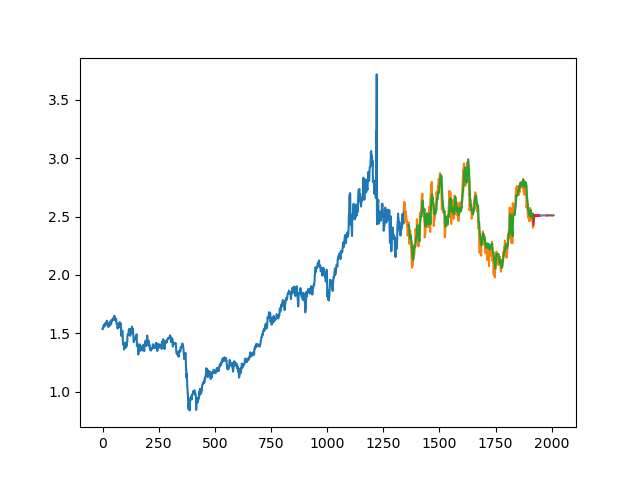
\includegraphics[width=0.8\textwidth]{Picture/RF/RF_Gasoline_RBOB_Week6.png}
    \caption{RF Gasoline RBOB 7:3}
    \label{fig:2}
    \end{minipage}
    \hfill
    \\
    \begin{minipage}{0.3\textwidth}
    \centering
    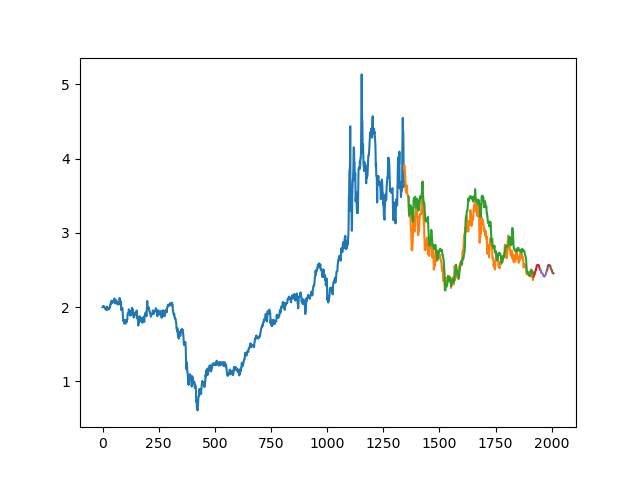
\includegraphics[width=0.8\textwidth]{Picture/RF/RF_Heating_Oil_Week6.png}
    \caption{RF Heating Oil 7:3}
    \label{fig:3}
    \end{minipage}
\end{figure}
\subsection{Long short-term memory (LSTM)}
LSTM là một loại đặc biệt của RNN với các tính năng bổ sung để ghi nhớ chuỗi dữ liệu. Việc ghi nhớ xu hướng trước đó của dữ liệu là có thể thông qua một số cổng cùng với một dòng bộ nhớ được tích hợp trong một LSTM điển hình.  

Hình dưới đây biểu diễn khối bộ nhớ của LSTM:
\begin{figure}[H]
    \centering
    \begin{minipage}{0.3\textwidth}
    \centering
    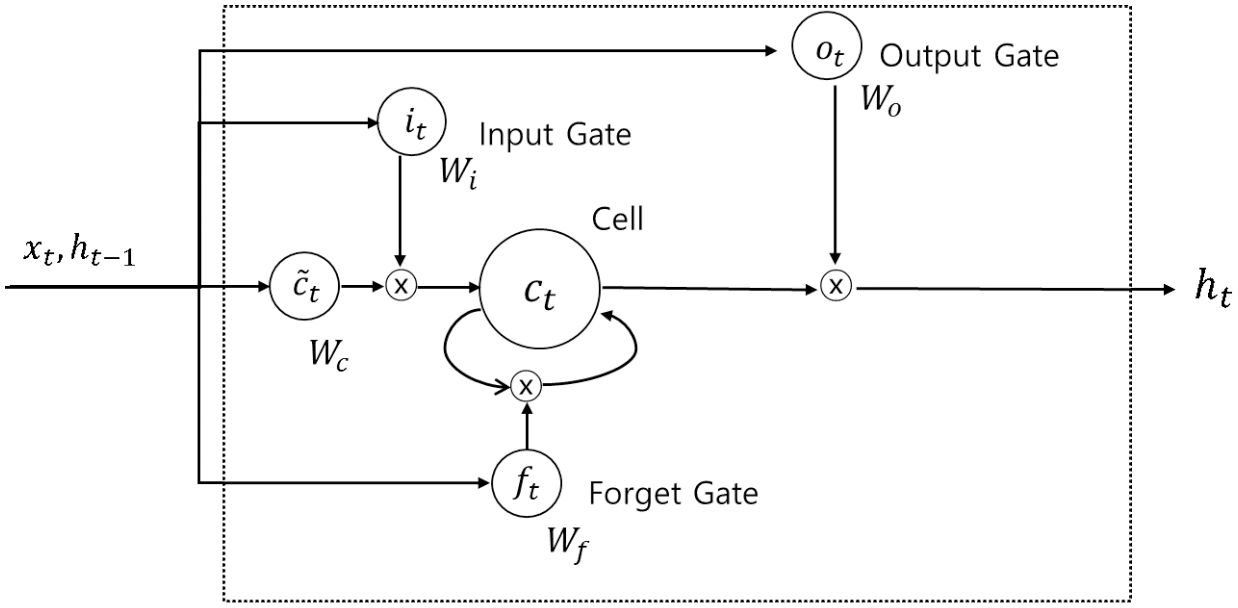
\includegraphics[width=0.8\textwidth]{Picture/LSTM/LSTM_pic.png} 
    \caption{Khối bộ nhớ của một LSTM}
    \label{fig:1}
    \end{minipage}
    \hfill
    \\
  
\end{figure}

Ba loại cổng được tham gia vào mỗi LSTM với mục tiêu kiểm soát trạng thái của từng ô:

\begin{itemize}
    \item Cổng Quên xuất ra một số giữa 0 và 1, trong đó 1 cho thấy "hoàn toàn giữ lại điều này"; trong khi 0 ngụ ý "hoàn toàn bỏ qua điều này".
    \item Cổng Bộ Nhớ chọn dữ liệu mới nào cần được lưu trữ trong ô. Đầu tiên, một lớp sigmoid, được gọi là "lớp cửa vào" chọn những giá trị nào sẽ được thay đổi. Tiếp theo, một lớp "tanh" tạo ra một vector các giá trị ứng viên mới có thể được thêm vào trạng thái.
    \item Cổng Đầu Ra quyết định những gì sẽ được xuất ra từ mỗi ô. Giá trị xuất ra sẽ dựa trên trạng thái ô cùng với dữ liệu được lọc và thêm mới. 
\end{itemize}

 Cụ thể, biểu thức toán học của LSTM được viết như sau:
 
1. Cổng Quên:
\[
f_t = \sigma(W_{xf} x_t + W_{hf} h_{t-1} + b_f)
\]

2. Cổng Bộ Nhớ:
\[
i_t = \sigma(W_{xi} x_t + W_{hi} h_{t-1} + b_i)
\]

3. Giá trị ứng viên mới:
\[
\tilde{c}_t = \tanh(W_{xc} x_t + W_{hc} h_{t-1} + b_c)
\]

4. Trạng thái ô hiện tại:
\[
c_t = f_t \ast c_{t-1} + i_t \ast \tilde{c}_t
\]

5. Cổng Đầu Ra:
\[
o_t = \sigma(W_{xo} x_t + W_{ho} h_{t-1} + b_o)
\]

6. Đầu ra ô:
\[
h_t = o_t \ast \tanh(c_t)
\]
\\
Trong đó: \( \sigma \) là hàm sigmoid, \( \tanh \) là hàm hyperbolic tangent, \( W \) là các ma trận trọng số, \( b \) là các hệ số bù, \( x_t \) là đầu vào tại thời điểm \( t \), \( h_{t-1} \) là đầu ra của ô tại thời điểm \( t-1 \), \( c_t \) là trạng thái ô tại thời điểm \( t \), \( f_t \) là đầu ra của cổng quên, \( i_t \) là đầu ra của cổng bộ nhớ, \( o_t \) là đầu ra của cổng đầu ra, \( \tilde{c}_t \) là giá trị ứng viên mới cho trạng thái ô.

Trong các phương trình (1) đến (6), các biến đầu vào \( x_t \) và \( h_{t-1} \) đi vào bốn cổng được gán nhãn là \( f_t \), \( i_t \),\( c_t \), \( o_t \). Đối với các cổng đầu vào và đầu ra, các trọng số tương ứng với mỗi cổng được tính toán, và hàm sigmoid được sử dụng làm hàm kích hoạt.

Hàm sigmoid lấy giá trị giữa 0 và 1. Nếu giá trị đầu ra là 1, giá trị tương ứng nên được giữ lại, nhưng nếu giá trị đầu ra là 0, giá trị tương ứng nên bị loại bỏ hoàn toàn. Đối với cổng còn lại, cổng điều chế đầu vào, hàm tanh được sử dụng để xác định lượng thông tin mới cần được phản ánh trong trạng thái ô. Cuối cùng, thông tin cần được phản ánh trong \( c_t \) được tính bằng cách cộng nhân điểm của các giá trị \( i_t \) đã tính toán trước đó và các giá trị được tính từ cổng quên, giá trị trạng thái ô trước đó, và nhân điểm của \( c_t \). 

Cuối cùng, để tính giá trị đầu ra \( h_t \), nhân điểm được thực hiện trên giá trị được tính từ cổng đầu ra và giá trị thu được bằng cách thêm hàm tanh vào giá trị trạng thái ô đã tính toán.



\begin{figure}[H]
    \centering
    \begin{minipage}{0.3\textwidth}
    \centering
    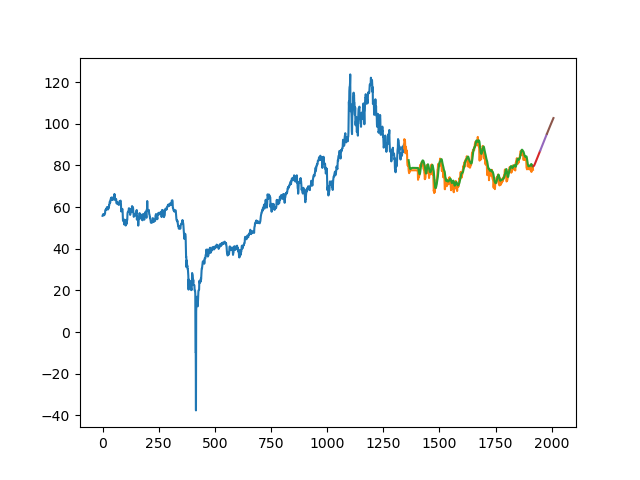
\includegraphics[width=0.8\textwidth]{Picture/LSTM/LSTM_Cruide_Oil_Week6.png} 
    \caption{LSTM Crude Oil WTI 7:3}
    \label{fig:1}
    \end{minipage}
    \hfill
    \\
    \begin{minipage}{0.3\textwidth} 
    \centering
    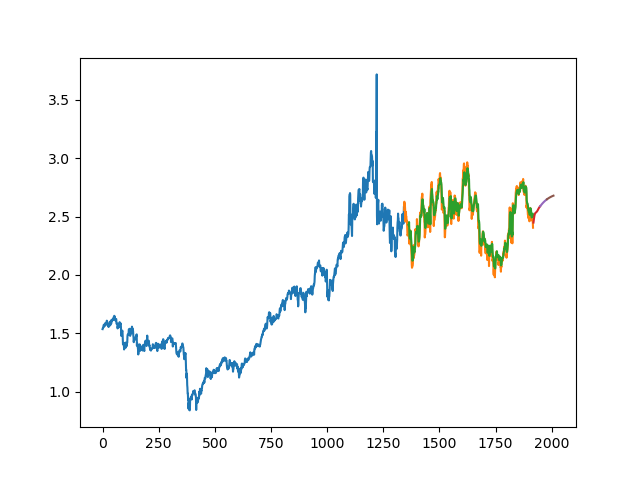
\includegraphics[width=0.8\textwidth]{Picture/LSTM/LSTM_Gasoline_RBOB_Week6.png}
    \caption{LSTM Gasoline RBOB 7:3}
    \label{fig:2}
    \end{minipage}
    \hfill
    \\
    \begin{minipage}{0.3\textwidth}
    \centering
    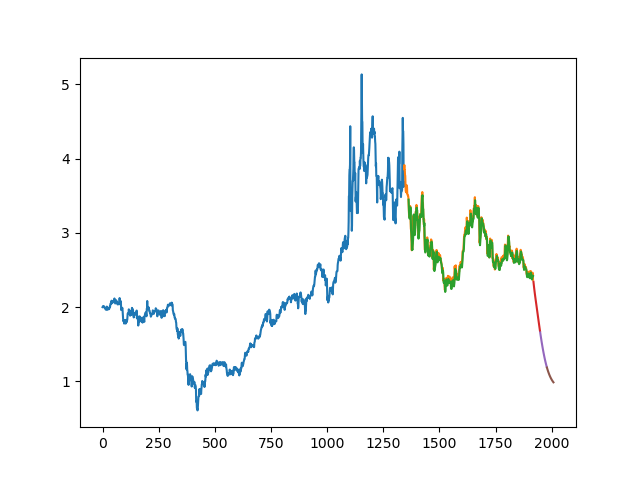
\includegraphics[width=0.8\textwidth]{Picture/LSTM/LSTM_Heating_Oil_Week6.png}
    \caption{LSTM Heating Oil 7:3}
    \label{fig:3}
    \end{minipage}
\end{figure}
\subsection{Dynamic Linear Model (DLM)}
Mô hình tuyến tính động (Dynamic Linear Model - DLM) là một thuật toán thống kê được sử dụng để mô hình hóa và dự đoán các chuỗi dữ liệu thời gian. Nó là một phần của lĩnh vực học máy thống kê và thường được sử dụng trong việc phân tích dữ liệu thời gian, dự báo, và điều khiển.
Một DLM bao gồm hai thành phần chính:
\begin{itemize}
    \item State component: Đây là một mô hình tuyến tính động mà mô tả sự phát triển của hệ thống theo thời gian. Mô hình trạng thái sử dụng các biến trạng thái để mô tả trạng thái hiện tại của hệ thống dựa trên trạng thái trước đó và các yếu tố biến đổi. Mô hình trạng thái thường được mô tả bằng một phương trình đệ quy.
    \item Observation component: Mô hình quan sát mô tả cách mà các biến trạng thái ảnh hưởng đến dữ liệu được thu thập trong thực tế. Thông thường, mô hình quan sát sử dụng một mô hình tuyến tính để liên kết giữa các biến trạng thái và các biến quan sát.
\end{itemize}
Phương trình trạng thái (State equation):
\[
\mathbf{x}_t = \mathbf{G}_t \mathbf{x}_{t-1} + \mathbf{w}_t
\]
Trong đó, $\mathbf{x}_t$ là vector trạng thái tại thời điểm $t$, $\mathbf{G}_t$ là ma trận chuyển tiếp trạng thái tại thời điểm $t$, và $\mathbf{w}_t$ là vector nhiễu trạng thái tại thời điểm $t$.

Phương trình quan sát (Observation equation)::
\[
\mathbf{y}_t = \mathbf{F}_t \mathbf{x}_t + \mathbf{v}_t
\]
Trong đó, $\mathbf{y}_t$ là vector quan sát tại thời điểm $t$, $\mathbf{F}_t$ là ma trận quan sát tại thời điểm $t$, và $\mathbf{v}_t$ là vector nhiễu quan sát tại thời điểm $t$.

\begin{figure}[H]
    \centering
    \begin{minipage}{0.3\textwidth}
    \centering
    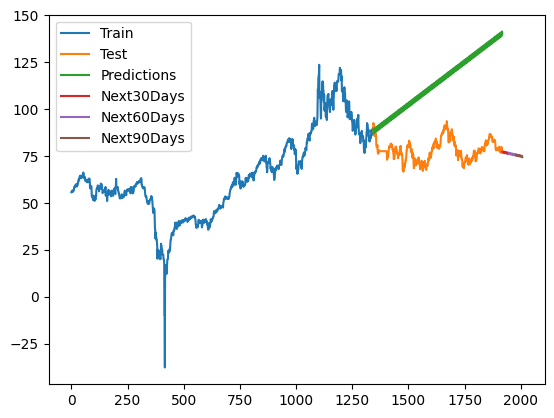
\includegraphics[width=0.8\textwidth]{Picture/DLM/DLM_Crude_73.png} 
    \caption{Crude Oil WTI 7:3}
    \label{fig:1}
    \end{minipage}
    \hfill
    \\
    \begin{minipage}{0.3\textwidth} 
    \centering
    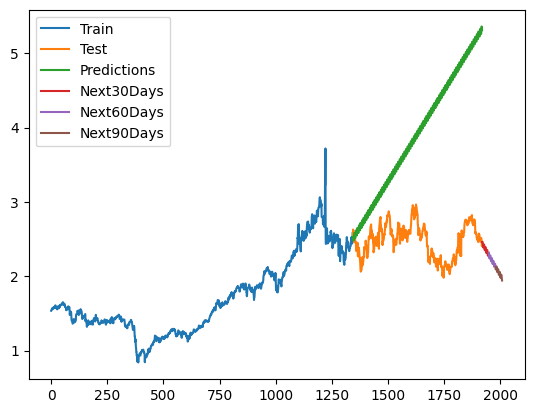
\includegraphics[width=0.8\textwidth]{Picture/DLM/DLM_Gasoline_73.png}
    \caption{Gasoline RBOB 7:3}
    \label{fig:2}
    \end{minipage}
    \hfill
    \\
    \begin{minipage}{0.3\textwidth}
    \centering
    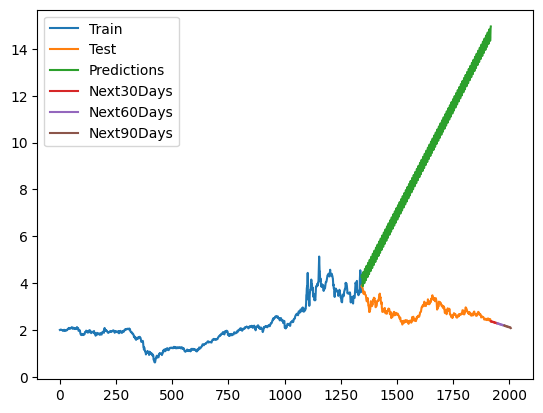
\includegraphics[width=0.8\textwidth]{Picture/DLM/DLM_Heating_73.png}
    \caption{Heating Oil 7:3}
    \label{fig:3}
    \end{minipage}
\end{figure}


\subsection{Gated Recurrent Unit (GRU)}
Gated Recurrent Unit (GRU) là một kiểu kiến trúc mạng nơ-ron hồi tiếp (RNN) được thiết kế để xử lý dữ liệu chuỗi. GRU được giới thiệu để giảm số lượng cổng so với mô hình Long Short-Term Memory (LSTM), giúp cho việc triển khai và huấn luyện trở nên đơn giản hơn. Dưới đây là một phần của kiến trúc GRU và các công thức tương ứng:

1. Cổng cập nhập (Update Gate):
Cổng cập nhật xác định bao nhiêu trạng thái ẩn trước
đó sẽ được giữ lại và bao nhiêu thông tin mới sẽ được đưa vào.
Nó được tính như sau:
\[
z_t = \sigma(W_z \cdot [h_{t-1}, x_t] + b_z)
\]
Trong đó, \( x_t \) là đầu vào tại thời điểm \( t \), \( h_{t-1} \) là trạng thái ẩn tại thời điểm trước đó, \( W_z \) là ma trận trọng số, \( b_z \) là vector bias, và \( \sigma \) là hàm kích hoạt sigmoid.
2. Trạng thái cập nhật: Trạng thái ẩn ứng viên được tính dựa trên đầu vào hiện tại và trạng thái ẩn trước đó.
\[
\tilde{h}_t = \text{tanh}(W_h \cdot [r_t \odot h_{t-1}, x_t] + b_h)
\]
Trong đó, \( r_t \) là cổng reset, và \( \odot \) biểu thị phép nhân theo từng phần tử.

3. Cổng reset : Quyết định mức độ thông tin nào sẽ bị xóa khỏi trạng thái ẩn trước khi tính toán trạng thái ẩn hiện tại.
\[ r_t = \sigma(W_r \cdot [h_{t-1}, x_t] + b_r) \]
4. Trạng thái ẩn mới: Tích hợp thông tin từ trạng thái ẩn trước và trạng thái ẩn hiện tại để tạo ra trạng thái ẩn mới.
   \[ h_t = (1 - z_t) \odot h_{t-1} + z_t \odot \tilde{h}_t \]

\begin{figure}[H]
    \centering
    \begin{minipage}{0.3\textwidth}
    \centering
    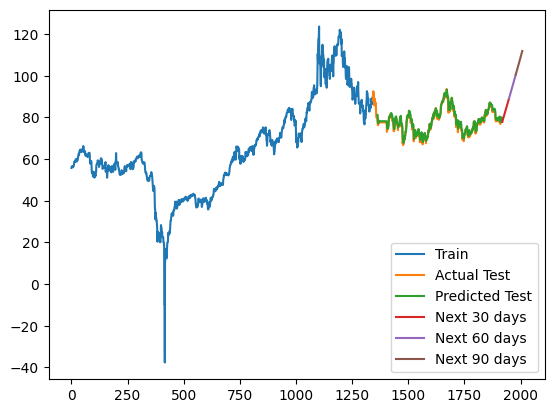
\includegraphics[width=0.8\textwidth]{Picture/GRU/GRU_Crude_73.png} 
    \caption{Crude Oil WTI 7:3}
    \label{fig:1}
    \end{minipage}
    \hfill
    \\
    \begin{minipage}{0.3\textwidth} 
    \centering
    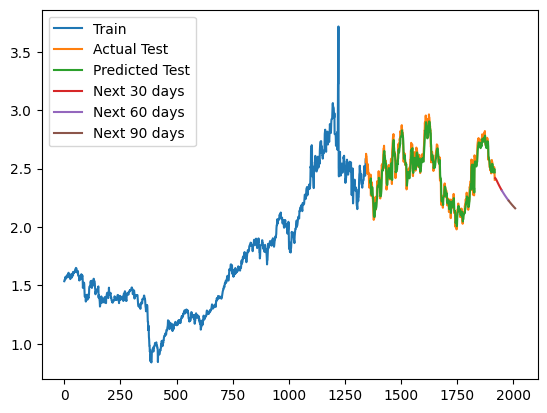
\includegraphics[width=0.8\textwidth]{Picture/GRU/GRU_Gasoline_73.png}
    \caption{Gasoline RBOB 7:3}
    \label{fig:2}
    \end{minipage}
    \hfill
    \\
    \begin{minipage}{0.3\textwidth}
    \centering
    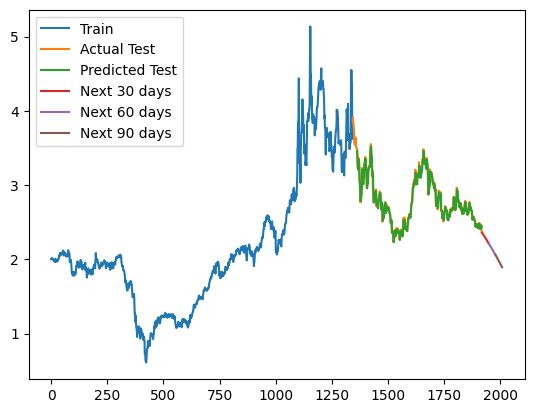
\includegraphics[width=0.8\textwidth]{Picture/GRU/GRU_Heating_73.png}
    \caption{Heating Oil 7:3}
    \label{fig:3}
    \end{minipage}
\end{figure}

\subsection{Additive Recurrent Neural Network (AddRNN)}

AddRNN là một phần mở rộng của Mạng nơ-ron hồi quy tiêu chuẩn (RNN), được thiết kế đặc biệt để giải quyết các thách thức do dữ liệu tuần tự đặt ra. Điểm đặc trưng chính của AddRNN là tính chất cộng thêm, trong đó đầu ra của mỗi đơn vị hồi quy là sự tích lũy của các trạng thái trước đó.

Cách tiếp cận cộng thêm này giúp nắm bắt các phụ thuộc dài hạn hiệu quả hơn so với RNN truyền thống.
 Sự đổi mới cốt lõi của AddRNN nằm ở cơ chế cộng thêm của nó. Thay vì đơn giản cập nhật trạng thái ẩn tại mỗi thời điểm, AddRNN thêm thông tin mới vào trạng thái trước đó, cho phép nó duy trì các phụ thuộc dài hạn mà không gặp rủi ro gradient biến mất. Quy tắc cập nhật cộng thêm có thể được mô tả như sau:
\[
H_t = H_{t-1} + f(U \cdot X_t + W \cdot H_{t-1} + b)
\]
Trong đó:\( X_t \) là đầu vào tại thời điểm \( t \), \( H_t \) là trạng thái ẩn tại thời điểm \( t \), \( H_{t-1} \) là trạng thái ẩn tại thời điểm \( t - 1 \), \( U \) là ma trận trọng số liên kết giữa đầu vào và trạng thái ẩn, \( W \) là ma trận trọng số liên kết giữa trạng thái ẩn tại thời điểm trước đó và trạng thái ẩn tại thời điểm hiện tại, \( b \) là vector độ lệch (bias), \( f \) là hàm kích hoạt.

Công thức này đảm bảo rằng trạng thái ẩn \(H_t\) là tổng cộng dồn của tất cả các trạng thái ẩn trước đó và đầu vào hiện tại. Sự tích lũy này cho phép mô hình duy trì và truyền tải thông tin quan trọng qua các chuỗi dài hơn.
Sự khác biệt chính giữa Mạng nơ-ron hồi quy thông thường (RNN) và Mạng nơ-ron hồi quy cộng thêm (AddRNN) nằm ở cách chúng xử lý các cập nhật trạng thái ẩn. 

Trong RNN thông thường, trạng thái ẩn tại mỗi thời điểm được thay thế hoàn toàn, điều này có thể gây khó khăn trong việc nắm bắt các phụ thuộc dài hạn do vấn đề gradient biến mất. Ngược lại, AddRNN sử dụng cơ chế cập nhật cộng thêm, trong đó trạng thái ẩn là tổng cộng dồn của tất cả các trạng thái trước đó và đầu vào hiện tại. Cách tiếp cận này cải thiện luồng gradient, giảm nguy cơ gradient biến mất và tăng cường khả năng nắm bắt các phụ thuộc dài hạn. 
\begin{figure}[H]
    \centering
    \begin{minipage}{0.3\textwidth}
    \centering    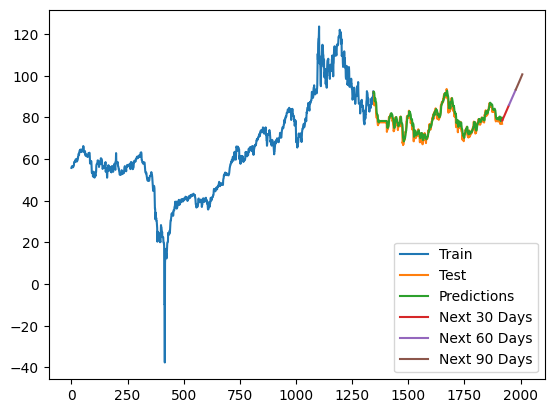
\includegraphics[width=0.8\textwidth]{Picture/AddRNN/Crude Oil WTI 7_3 AddRNN.png} 
    \caption{Crude Oil WTI 7:3}
    \label{fig:1}
    \end{minipage}
    \hfill
    \\
    \begin{minipage}{0.3\textwidth} 
    \centering
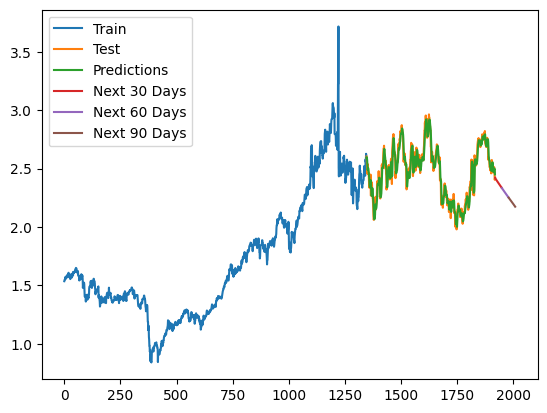
\includegraphics[width=0.8\textwidth]{Picture/AddRNN/Gasoline RBOB 7_3 AddRNN.png} 
    \caption{Gasoline RBOB 7:3}
    \label{fig:2}
    \end{minipage}
    \hfill
    \\
    \begin{minipage}{0.3\textwidth}
    \centering
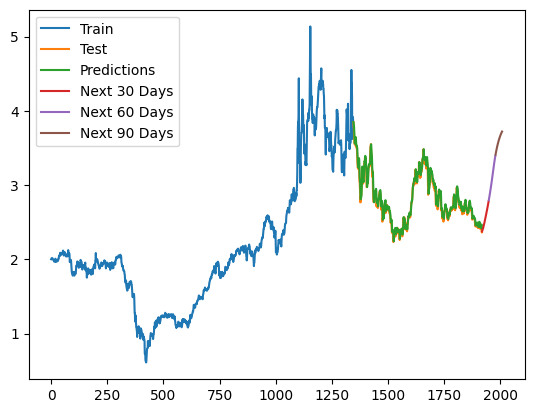
\includegraphics[width=0.8\textwidth]{Picture/AddRNN/Heating Oil 7_3 AddRNN.png}
    \caption{Heating Oil 7:3}
    \label{fig:3}
    \end{minipage}
\end{figure}
\par
\subsection{Fully Convolutional Neural Networks (FCN)}\par
Mô hình Fully Convolutional Neural Networks (FCN) lần đầu tiên được đề xuất trong công trình của Wang et al. (2017b). FCN là một loại mạng nơ-ron mà trong đó tất cả các lớp đều là lớp tích chập (convolutional layers), không có các lớp kết nối đầy đủ (fully connected layers). FCN được áp dụng vào chuỗi thời gian để trích xuất các đặc trưng quan trọng từ dữ liệu chuỗi thời gian. Quá trình này bao gồm các lớp tích chập, max-pooling để xây dựng mô hình có khả năng dự đoán hoặc phân loại chính xác các giá trị trong chuỗi thời gian. 

Công thức tổng quát của mô hình FCN cho chuỗi thời gian bao gồm các lớp tích chập (convolutional layers) và các lớp khác như max-pooling như mô tả sau:\\

\textbf{Lớp đầu vào (Input Layer)}
Đầu vào của mô hình FCN là một chuỗi thời gian đa chiều \( X \) có kích thước \( (N, C, L) \), trong đó:
\begin{itemize}
    \item \( N \) là số lượng mẫu trong batch.
    \item \( C \) là số lượng kênh (channels) hoặc các đặc trưng đầu vào.
    \item \( L \) là chiều dài của chuỗi thời gian.
\end{itemize}

\textbf{Các lớp tích chập (Convolutional Layers)}
Các lớp tích chập liên tiếp được áp dụng để trích xuất các đặc trưng từ chuỗi thời gian. Một lớp tích chập cơ bản có thể được biểu diễn như sau:
\[
Z_i = f(W_i * X + b_i)
\]
Trong đó: \( Z_i \) là đầu ra của lớp tích chập thứ \( i \),
    \( W_i \) là trọng số của bộ lọc (filter) trong lớp tích chập thứ \( i \),
    \( * \) là phép tích chập,
    \( b_i \) là bias của lớp tích chập thứ \( i \),
    \( f \) là hàm kích hoạt (activation function), chẳng hạn như ReLU (Rectified Linear Unit).
\\

\textbf{Các lớp gộp (Pooling Layers)}
Đôi khi, sau một hoặc nhiều lớp tích chập, một lớp gộp (pooling layer) được áp dụng để giảm chiều không gian và tổng hợp các đặc trưng. Max Pooling là một ví dụ phổ biến:
\[
P_i = \text{MaxPooling}(Z_i)
\]
\\
Trong đó:
 \( P_i \) là đầu ra của lớp gộp thứ \( i \).\\


\textbf{Lớp gộp trung bình toàn cục (Global Average Pooling)}
Trước khi đến lớp đầu ra, một lớp Global Average Pooling (GAP) hoặc Global Max Pooling (GMP) thường được sử dụng để tổng hợp các đặc trưng không gian thành một vector duy nhất:
\[
G = \text{GlobalAveragePooling}(P_n)
\]
hoặc
\[
G = \text{GlobalMaxPooling}(P_n)
\]
Trong đó: \( P_n \) là đầu ra của lớp gộp cuối cùng.
\\

\textbf{Lớp đầu ra (Output Layer)}
Lớp đầu ra là một lớp tích chập với kích thước đầu ra phù hợp với bài toán cần giải quyết (ví dụ: số lượng lớp trong bài toán phân loại hoặc số lượng đơn vị trong bài toán hồi quy).

Đối với bài toán phân loại, lớp đầu ra có thể sử dụng hàm softmax hoặc sigmoid tùy thuộc vào số lượng lớp:
\[
\hat{y} = \text{softmax}(W_o * G + b_o)
\]
hoặc
\[
\hat{y} = \text{sigmoid}(W_o * G + b_o)
\]
\\
Trong đó:
 \( W_o \) là trọng số của lớp đầu ra,
 \( b_o \) là bias của lớp đầu ra.
\\
\begin{figure}[H]
    \centering
    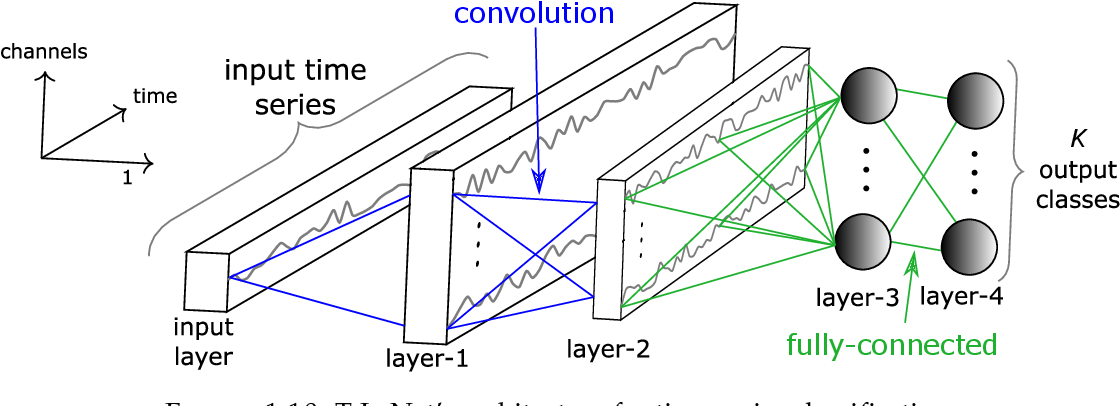
\includegraphics[width=0.5\textwidth]{Picture/FCN/FCN_structure.png} 
    \caption{Cấu trúc mô hình FCN}
\end{figure}

\begin{figure}[H]
    \centering
    \begin{minipage}{0.3\textwidth}
    \centering
    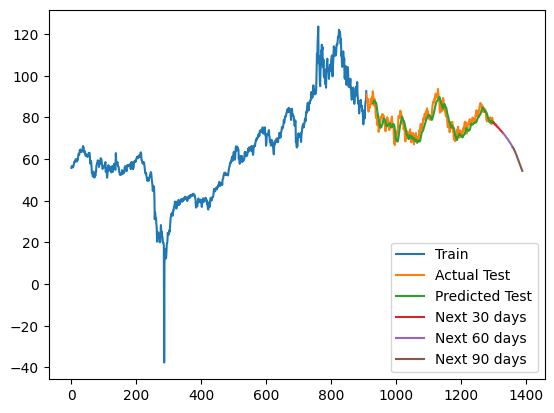
\includegraphics[width=0.8\textwidth]{Picture/FCN/FCN_Cruide_7_3.png} 
    \caption{Crude Oil WTI 7:3}
    \label{fig:1}
    \end{minipage}
    \hfill
    \\
    \begin{minipage}{0.3\textwidth} 
    \centering
    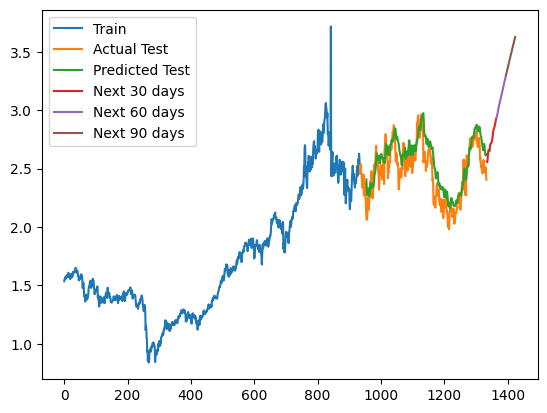
\includegraphics[width=0.8\textwidth]{Picture/FCN/FCN_Gao_7_3.png} 
    \caption{Gasoline RBOB 7:3}
    \label{fig:2}
    \end{minipage}
    \hfill
    \\
    \begin{minipage}{0.3\textwidth}
    \centering
    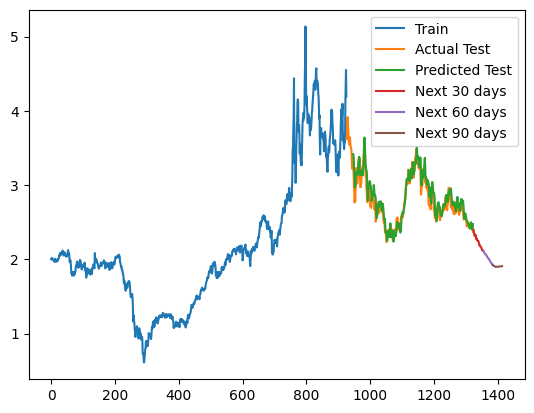
\includegraphics[width=0.8\textwidth]{Picture/FCN/FCN_Heating_7_3.png}
    \caption{Heating Oil 7:3}
    \label{fig:3}
    \end{minipage}
\end{figure}
\section*{KẾT QUẢ THỰC NGHIỆM}

Kết quả đánh giá thực nghiệm trên 3 bộ dữ liệu được thể hiện ở Bảng II bên dưới. Ghi nhận lại các giá trị độ đo RMSE, MAPE, MAE được làm tròn tới hai chữ số thập phân của các mô hình  trên tập test của 3 bộ dữ liệu về giá Crude OIL, Gasoline RBOB, Heating OIL theo 3 tỉ lệ là 7:3, 8:2, 9:1.

Xét giá trị nhỏ nhất khi chưa làm tròn của mỗi độ đo RMSE, MAPE và MAE được đánh dấu bằng màu đỏ, các chỉ số độ đo càng thấp thể hiện các mô hình có giá trị tốt nhất trên từng bộ dữ liệu và từng tỉ lệ train.

Trong số 10 mô hình được xem xét, mô hình Gated Recurrent Unit (GRU) đạt được nhiều giá trị nhất nhất trong bộ dữ liệu Heating OIL ở cả ba tỉ lệ train
. Ngoài ra, GRU cũng chiếm ưu thế với nhiều giá trị nhỏ nhất trong các bộ dữ liệu khác như Gasoline RBOB với tỉ lệ train
8:2 và 9:1, cũng như đạt giá trị MAPE nhỏ nhất trong bộ dữ liệu Crude OIL.

Mặt khác, mô hình Fast Fourier Transform Forecasting Model (FFT) cho kết quả tốt nhất trong bộ dữ liệu Crude OIL với các giá trị độ đo RMSE và MAE nhỏ nhất ở cả ba tỉ lệ train.

Trong trường hợp của RNN chỉ cho kết quả tốt nhất ở hai độ đo RMSE và MAE trong dataset duy nhất với tỉ lệ train:test (7:3).

Tổng Kết lại nhóm nhận thấy được model tốt nhất để thực hiện dự đoán giá của nhiên liệu là Gated Recurrent Unit (GRU).
\section*{KẾT LUẬN}

Thông qua bài báo cáo này, chúng tôi đã tiến hành nghiên cứu về việc sử dụng các mô hình máy học và học sâu để phân tích chuỗi thời gian nhằm dự đoán giá của các loại nhiên liệu. Chúng tôi sử dụng các mô hình như Linear Regression, ARIMA, FFT, Random Forest, DLM, LSTM, RNN, GRU, FCN và AddRNN trên ba bộ dữ liệu khác nhau để đưa ra đánh giá các mô hình và dự đoán giá trong tương lai. Việc này chỉ ra được sự phù hợp trong việc dự đoán giá của nhiên liệu của mô hình dựa trên mạng nơ-ron hồi quy và kỹ thuật chuỗi thời gian.

Trong quá trình nghiên cứu việc gặp khó khăn là không thể tránh khỏi. Việc khó khăn nhất chính là sự phức tạp biến động mạnh của thị trường. Làm tăng độ khó của việc dự đoán giá nhiên liệu.

Trong tương lai việc cải tiến các mô hình nhằm tối ưu nhất trong việc dự đoán. Chúng tôi có thể sẽ áp dụng các công nghệ nghiên cứu mới hoặc các mô hình mới khác nhau nhằm tăng cao độ chính xác và tin cậy cho dự đoán.
\newpage
\begin{longtable}{|l|l|*{9}{>{\centering\arraybackslash}m{1.2cm}|}} % Adjust width as needed
    \caption{Kết quả đánh giá 10 mô hình dự đoán thông qua các độ đo } \label{tab:dataset-comparison} \\
    \hline
    Mô Hình & Độ đo & \multicolumn{3}{c|}{Crude OIL} & \multicolumn{3}{c|}{Gasoline RBOB} & \multicolumn{3}{c|}{Heating OIL} \\ \cline{3-11}
    && 7:3 & 8:2 & 9:1 & 7:3 & 8:2 & 9:1 & 7:3 & 8:2 & 9:1 \\ \hline
    \endfirsthead
    \endhead
    \hline    
    \multirow{3}{*}{\textbf{LN}} & RMSE & 25.4032 & 20.2504 & 17.072 & 0.3766 & 0.4332 & 0.4538 & 0.9667 & 0.9041 & 0.825 \\ \cline{2-11}
    & MAPE & 30.8304 & 25.0885 & 21.7823 & 12.5527 & 15.618 & 17.7105 & 32.5566 & 31.8655 & 30.7701 \\ \cline{2-11}
    & MAE & 23.7514 & 19.2747 & 16.725 & 0.2929 & 0.3618 & 0.4028 & 0.8706 & 0.8378 & 0.8061 \\ \hline
    \multirow{3}{*}{\textbf{FCN}} & RMSE & 2.9362 & 1.9562 & 1.6427 & 0.1015 & 0.0782 & 0.0732 & 0.1147 & 0.0633 & 0.063 \\ \cline{2-11}
    & MAPE & 2.98 & 1.9707 & 1.6296 & 3.267 & 2.4474 & 2.1855 & 4.0814 & 1.7337 & 1.837 \\ \cline{2-11}
    & MAE & 2.336 & 1.5608 & 1.2689 & 0.08 & 0.0599 & 0.0535 & 0.1147 & 0.0483 & 0.0483 \\ \hline
    \multirow{3}{*}{\textbf{ARIMA}} & RMSE & 12.5311 & 9.4956 & 4.3784 & 0.2296 & 0.2426 & 0.318 & 0.9004 & 0.4908 & 0.2885 \\ \cline{2-11}
    & MAPE & 15.0849 & 9.3863 & 4.6014 & 7.7550 & 8.7286 & 10.0869 & 31.5659 & 13.8670 & 10.1170 \\ \cline{2-11}
    & MAE & 11.3824 & 7.7245 & 3.5660 & 0.1837 & 0.2137 & 0.2584 & 0.8414 & 0.4045 & 0.2611 \\ \hline
    \multirow{3}{*}{\textbf{AddRNN}} & RMSE & 1.7352 & 2.2424 & 1.3570 & 0.0609 & 0.0542 & 0.0549 & 0.0617 & {0.0513} & {0.0381} \\ \cline{2-11}
    & MAPE & 1.6556 & 2.5050 & 1.4445 & 1.8206 & 1.6359 & 1.6017 & 1.6013 & 1.4342 & 1.0038 \\ \cline{2-11}
    & MAE & 1.2772 & 1.9676 & 1.1190 & 0.0448 & 0.0406 & 0.0379 & {0.0453} & {0.0393} & {0.0267} \\ \hline
    \multirow{3}{*}{\textbf{RNN}} & RMSE & 2.2993 & 1.3007 & 1.3271 & \textcolor{red}{0.0589} & 0.0564 & 0.0635 & 0.0646 & 0.0804 & 0.0388 \\ \cline{2-11}
    & MAPE & 2.5640 & 1.2527 & 1.3904 & 1.7695 & 1.7112 & 1.9388 & 1.6570 & 2.5523 & 1.1312 \\ \cline{2-11}
    & MAE & 1.9800 & 0.9795 & 1.0883 & \textcolor{red}{0.0441} & 0.0425 & 0.0479 & 0.0469 & 0.0703 & 0.0299 \\ \hline
    \multirow{3}{*}{\textbf{FFT}} & RMSE & \textcolor{red}{0.2006} & \textcolor{red}{0.1612} & \textcolor{red}{0.1364} & 0.4077 & 0.3684 & 0.3273 & 0.2771 & 0.2074 & 0.1343 \\ \cline{2-11}
    & MAPE & 24.9804 & 19.5114 & 16.3358 & 69.4313 & 61.6176 & 52.5137 & 53.4538& 39.9352 & 27.5730\\ \cline{2-11}
    & MAE & \textcolor{red}{0.1805} & \textcolor{red}{0.1428} & \textcolor{red}{0.1189} & 0.3966 & 0.3526 & 0.3008 & 0.2603 & 0.1926 & 0.1241 \\ \hline
    \multirow{3}{*}{\textbf{GRU}} & RMSE & 1.3203 &	1.2508 &	0.9916&0.0550&	\textcolor{red}{0.0505}&	\textcolor{red}{0.0488}&	\textcolor{red}{0.0533}&	\textcolor{red}{0.0458}&\textcolor{red}{0.0380}
 \\ \cline{2-11}
    & MAPE & \textcolor{red}{1.2853}&	\textcolor{red}{1.2271}&\textcolor{red}{0.9315}&	\textcolor{red}{1.6284}&	\textcolor{red}{1.4543}&	\textcolor{red}{1.2195}&\textcolor{red}{1.3442}&\textcolor{red}{1.1508}&	\textcolor{red}{1.0881}
 \\ \cline{2-11}
    & MAE & 0.9884 & 0.9641 & 0.7198&	0.0404 &	\textcolor{red}{0.0352}&	\textcolor{red}{0.0296}&	\textcolor{red}{0.0379}&	\textcolor{red}{0.0322}&	\textcolor{red}{0.0289}
 \\ \hline
    \multirow{3}{*}{\textbf{DLM}} & RMSE & 39.1372&	59.644&34.7311&	1.6629&	1.7929&	0.7181&	7.3617&	2.1031&	0.8699
 \\ \cline{2-11}
    & MAPE & 46.5439&	66.3445&36.5604&	59.1387&	63.4383&	22.9093&	244.0466&	69.9487&	28.8303
 \\ \cline{2-11}
    & MAE & 35.9866&	52.7018&	29.1815&	1.4293&	1.5671&	0.5890&6.6169&	1.9216&	0.7539    
 \\ \hline
    \multirow{3}{*}{\textbf{LSTM}} & RMSE & 2.4510& 2.0611& 1.3251& 0.0594& 0.0549& 0.0517& 0.0606& 0.0556& 0.0674 \\ \cline{2-11}
    & MAPE & 2.4611& 2.0306& 1.3264& 1.8064& 1.6946& 1.4052& 1.7006& 1.5329& 2.2615 \\ \cline{2-11}
    & MAE & 1.8883& 1.5821& 1.0288& 0.0441& 0.0421& 0.0343& 0.0474& 0.0429& 0.0599 \\ \hline
    \multirow{3}{*}{\textbf{RF}} & RMSE & 2.0151& 1.4925& 1.2606& 0.0875& 0.0749& 0.0685& 0.2180& 0.0694& 0.0493 \\ \cline{2-11}
    & MAPE & 1.9557& 1.4607& 1.2745& 2.7978& 2.3529& 2.0317& 5.9506& 1.8592& 1.3572 \\ \cline{2-11}
    & MAE & 1.5290& 1.1530& 0.9893& 0.0686& 0.0570& 0.0496& 0.1685& 0.0522& 0.0360 \\ \hline
\end{longtable}
\section*{Lời cảm ơn}
Chúng tôi xin gửi lời cảm ơn chân thành đến PGS. TS. Nguyễn Đình Thuân và Kỹ sư Nguyễn Minh Nhựt vì sự hướng dẫn trong quá trình thực hiện bài báo này. Sự chỉ dẫn chuyên môn và kiến thức sâu rộng của họ đã giúp chúng tôi nắm vững kỹ thuật phân tích chuỗi thời gian và dự đoán giá cổ phiếu.\\
Chúng tôi cũng cảm ơn các thành viên trong nhóm nghiên cứu vì sự hợp tác và hỗ trợ, tạo nên một môi trường làm việc tích cực và sáng tạo. Những đóng góp và thảo luận của nhóm đã giúp bài báo hoàn thiện hơn.\\
Cuối cùng, chúng tôi cảm ơn cả những người đã hỗ trợ và đóng góp vào thành công của bài báo này, góp phần quan trọng vào lĩnh vực nghiên cứu dự đoán giá cổ phiếu. Chúng tôi hy vọng công trình này sẽ tiếp tục được phát triển và ứng dụng rộng rãi.

\begin{thebibliography}
    {}
    \bibitem{b1} C. C. Emioma1 \& S. O. Edeki1 (2020) "Stock price prediction using machine learning on least-squares linear regression basis"
    \\
    \bibitem{b2} Chris Kuo/Dr. Dataman (2020) "A Technical Guide on RNN/LSTM/GRU for Stock Price Prediction."
    \\
    \\
    \\
    \\
    \\
    \\
    \\
    \\
    \\
    \\
    \\
    \\
    \\
    \\
    \\
    \\
    \\
    \\
    \\
    \\
    \\
    \\
    \\
    \\
    \\
    \\
    \\
    \\
    \\
    \\
    \\
    \\
    \\
    \\
    \\
    \\
    \\
    \\
    \\
    \\
    \\
    \\
    \\
    \\
    \\
    \\
    \\
    \\
    \\
    \\
    \bibitem{b3} B/O Trading Blog (2023) "Using the Random Forest ML Algorithm for Stock Price Prediction (Python Tutorial)"
    \\
    \bibitem{b4} Jialin Liu, Fei Chao, Yu-Chen Lin \& Chih-Min Lin (2019) "Stock Prices Prediction using Deep Learning Models"
    \\
    \bibitem{b5} Hassan Ismail Fawaz, Germain Forestier, Jonathan Weber, Lhassane Idoumghar \& Pierre-Alain Muller (2019) "Deep learning for time series classification: a review"
    \\
    \bibitem{b6} Colin Bonatti, Bekim Berisha \& Dirk Mohr (2022) "From CP-FFT to CP-RNN: Recurrent neural network surrogate model of crystal plasticity"
    \\
    \bibitem{b7} Semin Kwak \& Nikolas Geroliminis (2020) "Travel Time Prediction for Congested Freeways With a Dynamic Linear Model"
    \\
    \bibitem{b8} Statisticshowto.com "RMSE: Root Mean Square Error"
    \\
    \bibitem{b9} Statisticshowto.com "Mean Absolute Percentage Error (MAPE)"
    \\
    \bibitem{b10} Statisticshowto.com "Absolute Error \& Mean Absolute Error (MAE)"
\end{thebibliography}
\end{document}

